\documentclass[a4,portraitt]{slides}
\usepackage{biggy,graphicx,times}
\usepackage{tikz}

\addtolength{\topmargin}{-0.75in}
\title{COMSM1201 Further Lectures}

\begin{document}

\begin{center}
{\Large
COMSM1201\\
Algorithms \& Data Structures
}

Dr. Neill Campbell

Room 3.14 MVB

Neill.Campbell@bristol.ac.uk\\[1cm]

\end{center}

\newpage
{\samepage
{\Large
\begin{center}
{\Large{\bf Simple Recursion}}
\end{center}
\begin{itemize}
\item  When a function calls itself, this is known as recursion.
\item This is an important theme in Computer Science that crops up
time \& time again.
\item Can sometimes lead to very simple and elegant programs.
\end{itemize}
}
}

\newpage
{\samepage
{\large
\begin{center}
{\Large{\bf Fibonacci Sequences}}
\end{center}
A well known example of a recursive function is the Fibonacci
sequence. The first term is 1, the second term is 1 and each
successive term is defined to be the sum of the two previous
terms, i.e. :
\begin{verbatim}
fib(1) is 1
fib(2) is 1
fib(n) is fib(n-1)+fib(n-2)

1,1,2,3,5,8,13,21, ...
\end{verbatim}
}
}

\newpage
{\samepage
\begin{center}
{\Large{\bf Iteration \& Fibonacci Sequences}}
\end{center}
\begin{verbatim}
#include <stdio.h>

int fibonacci(int n);

int main(void)
{

   int i;

   for(i=1; i<45; i++){
      printf("%d = %d\n", i, fibonacci(i));
   }

   return 0;

}
\end{verbatim}
}

\newpage
{\samepage
\begin{center}
{\Large{\bf Iteration \& Fibonacci Sequences}}
\end{center}
\begin{verbatim}
int fibonacci(int n)
{
                                                                                          
   int i, a, b, next;
   if(n <= 2){
      return 1;
   }
                                                                                          
   a = 1; b = 1;                                                                          
   for(i=3; i<=n; i++){
      next = a + b;
      a = b;
      b = next;
   }
   return b;
}
\end{verbatim}
}

\newpage
{\samepage
\begin{center}
{\Large{\bf Recursive Fibonacci Sequence}}
\end{center}
\begin{verbatim}
int fibon(int n)
{

   if(n == 1) return 1;
   if(n == 2) return 1;

   return( fibon(n-1)+fibon(n-2));

}
\end{verbatim}
}

\newpage
{\samepage
\begin{center}
{\Large{\bf Iterative String Reverse}}
\end{center}
{\small
\begin{verbatim}
#include <stdio.h>
#include <string.h>

#define SWAP(A,B)
        {char temp; temp=A;A=B;B=temp;}

void Reverse_String(char *s, int n);

int main(void)
{

   char str[] = "Hello World!";

   Reverse_String(str, strlen(str));
   printf("%s\n", str);
   return 0;
}

/* Iterative Inplace String Reverse */
void Reverse_String(char *s, int n)
{
   int i, j;

   for(i=0, j=n-1; i<j; i++, j--){
       SWAP(s[i], s[j]);
   }
}
\end{verbatim}
}}

\newpage
{\samepage
\begin{center}
{\Large{\bf Recursive String Reverse}}
\end{center}
{\small
\begin{verbatim}
#include <stdio.h>
#include <string.h>

#define SWAP(A,B) {char temp; temp=A;A=B;B=temp;}

void Reverse_String(char *s, int start, int end);

int main(void)
{

   char str[]= "ABCDEFGHIJKLMNOPQRSTUVWXYZ";

   Reverse_String(str, 0, strlen(str)-1);
   printf("%s\n", str);

}

/* RECURSIVE : Inplace String Reverse */
void Reverse_String(char *s, int start, int end)
{
   if(start >= end){
      return;
   }
   SWAP(s[start], s[end]);
   Reverse_String(s, start+1, end-1);

}
\end{verbatim}
}
}

\newpage
{\samepage
\begin{center}
{\Large{\bf Output}}
\end{center}
{\small
\begin{verbatim}

Reverse String -->ABCDEFGHIJKLMNOPQRSTUVWXYZ<--
Reverse String -->ZBCDEFGHIJKLMNOPQRSTUVWXYA<--
Reverse String -->ZYCDEFGHIJKLMNOPQRSTUVWXBA<--
Reverse String -->ZYXDEFGHIJKLMNOPQRSTUVWCBA<--
Reverse String -->ZYXWEFGHIJKLMNOPQRSTUVDCBA<--
Reverse String -->ZYXWVFGHIJKLMNOPQRSTUEDCBA<--
Reverse String -->ZYXWVUGHIJKLMNOPQRSTFEDCBA<--
Reverse String -->ZYXWVUTHIJKLMNOPQRSGFEDCBA<--
Reverse String -->ZYXWVUTSIJKLMNOPQRHGFEDCBA<--
Reverse String -->ZYXWVUTSRJKLMNOPQIHGFEDCBA<--
Reverse String -->ZYXWVUTSRQKLMNOPJIHGFEDCBA<--
Reverse String -->ZYXWVUTSRQPLMNOKJIHGFEDCBA<--
Reverse String -->ZYXWVUTSRQPOMNLKJIHGFEDCBA<--
ZYXWVUTSRQPONMLKJIHGFEDCBA
\end{verbatim}
}
}

\newpage
{\samepage
\begin{center}
{\Large{\bf The Ubiquitous Maze}}
\end{center}
The correct route through a maze can often be obtained via
recursive rather than iterative methods.
{\huge
\begin{center}
\verb^#.###^\\
\verb^#...#^\\
\verb^###.#^\\
\verb^#...#^\\
\verb^#X###^
\end{center}
}
\strut\\[0.2cm]
{\small
\begin{verbatim}
int explore(int x, int y, char mz[YS][XS])
{

   if  mz[y][x] is exit return 1;

   Mark mz[y][x] so we don't return here

   if we can go up :
      if(explore(x, y+1, mz)) return 1

   if we can go right :
      if(explore(x+1, y, mz)) return 1

   Do left & down in a similar manner

   return 0; /* Failed to find route */

}
\end{verbatim}
}}

\newpage
{\samepage
\begin{center}
{\Large{\bf Permuting}}
\end{center}
{\small
\begin{verbatim}
/* Borrowed from e.g.
   http://www.geeksforgeeks.org
*/
#include <stdio.h>
#include <string.h>

int main()
{
    char str[] = "ABC";
    int n = strlen(str);
    permute(str, 0, n-1);
    return 0;
}
 
void permute(char *a, int l, int r)
{
   int i;
   if (l == r){
     printf("%s\n", a);
     return;
   }
   for (i = l; i <= r; i++){
      swap((a+l), (a+i));
      permute(a, l+1, r);
      swap((a+l), (a+i)); /*backtrack*/
   }
}
\end{verbatim}
}}

\newpage
{\samepage
\begin{center}
{\Large{\bf Power}}
\end{center}
{\small
\begin{verbatim}
/* Try to write power(a,b) to computer a^b
   without using any maths functions other than
   multiplication :
   Try (1) iterative then (2) recursive
   (3) Trick that for n%2==0, x^n = x^(n/2)*x^(n/2)

*/

#include <stdio.h>

int power(unsigned int a, unsigned int b);

int main(void)
{

   int x = 2;
   int y = 16;

   printf("%d^%d = %d\n", x, y, power(x,y));

}

int power(unsigned int a, unsigned int b)
{
}
\end{verbatim}
}}

\newpage
{\samepage
\begin{center}
{\Large{\bf Simple Searching}}
\end{center}
{\large
\begin{itemize}
\item The need to search an array for a particular value is a common problem.
\item This is used to delete names from a mailing list,
or upgrading the salary of an employee etc.
\item The simplest method for searching is called the sequential search.
\item Simply move through the array from beginning to end,
stopping when you have found the value you require.
\end{itemize}
}
}

\newpage
{\samepage
\begin{center}
{\Large{\bf Sequential Search 1}}
\end{center}
{\small
\begin{verbatim}
#include <stdio.h>
#include <string.h>

#define NOTFOUND -1
#define NUMPEOPLE 6

struct person{
        char *name;
        int age;
};

typedef struct person Person;

int FindAge(char *name, Person *l, int n);

int main(void)
{
   Person ppl[NUMPEOPLE] = {
              {"Ackerby", 21}, {"Bloggs", 25},
              {"Chumley", 26}, {"Dalton",   25},
              {"Eggson", 22}, {"Fulton",  41} };

   printf("%d\n", FindAge("Eggson",   ppl, NUMPEOPLE));
   printf("%d\n", FindAge("Campbell", ppl, NUMPEOPLE));

   return 0;
}
\end{verbatim}
}}

\newpage
{\samepage
\begin{center}
{\Large{\bf Sequential Search 2}}
\end{center}
\begin{verbatim}
int FindAge(char *name, Person *p, int n)
{
   int j;
   for(j=0; j<n; j++){
      if(strcmp(name, p[j].name) == 0){
         return p[j].age;
      }
   }

   return NOTFOUND;
}
\end{verbatim}
}

\newpage
{\samepage
\begin{center}
{\Large{\bf Ordered Sequential Search}}
\end{center}
\begin{itemize}
\item {\bf If} we know that the array is ordered on the basis of names, then we can stop searching once the search key is alphabetically greater than the item at the current position in the list.
\item In large lists this can save an enormous amount of time.
\end{itemize}
\begin{verbatim}
int FindAge(char *name, Person *p, int n)
{
   int j, m;

   for(j=0; j<n; j++){
      m = strcmp(name, p[j].name);
      if(m == 0)
         return p[j].age;
      if(m < 0)
         return NOTFOUND;
   }
   return NOTFOUND;
}
\end{verbatim}
}

\newpage
{\samepage
\begin{center}
{\Large{\bf Binary Search for ``101''}}
\end{center}
\begin{itemize}
\item Searching small lists doesn't require much computation time.
\item However, as lists get longer (e.g. phone directories), sequential searching becomes extremely inefficient.
\item A binary search consists of examining the middle element of the array to see if it has the desired value. If not, then half the array may be discarded for the next search.
\end{itemize}
{\tiny
\[
\begin{array}{cccccccccccccc}
\\
\\
4 & 7 & 19 & 25 & 36 & 37 & 50 & 100 & 101 & 205 & 220 & 270 & 301 & 321 \\
\\
\\
\Uparrow & & & & & & \uparrow & & & & & & & \Uparrow \\
\\
\\
& & & & & & & \Uparrow & & & \uparrow & & & \Uparrow \\
\\
\\
& & & & & & & \Uparrow & \uparrow & \Uparrow & & & & \\
\end{array}
\]
}
}

\newpage
{\samepage
\begin{center}
{\Large{\bf Driver Function}}
\end{center}
{\small
\begin{verbatim}
#include <stdio.h>
#include <stdlib.h>
#include <assert.h>
#include <time.h>
#define NMBRS 1000000

int bin_it(int k, int *a, int l, int r);

int main(void)
{
   int i, n;
   int a[NMBRS];
   srand(time(NULL));
   for(i=0; i<NMBRS; i++){
      a[i] = 2*i;
   }
   for(i=0; i<10*NMBRS; i++){
      n=bin_it(a[rand()%NMBRS], a, 0, NMBRS-1);
      assert(n >= 0);
   }
   return 0;
}
\end{verbatim}
}}

\newpage
{\samepage
\begin{center}
{\Large{\bf Iterative Binary Search}}
\end{center}
\begin{verbatim}
int bin_it(int k, int *a, int l, int r)
{
   int m;
   while(l <= r){
      m = (l+r)/2;
      if(k == a[m]){
         return m;
      }
      else{
         if (k > a[m]){
            l = m + 1;
         }
         else{
            r = m- 1;
         }
      }
   }
   return -1;
}
\end{verbatim}
}

\newpage
{\samepage
\begin{center}
{\Large{\bf Recursive Binary Search}}
\end{center}
\begin{itemize}
\item Much of the processing in the previous function was controlled by a  while() loop.
\item We now know how to replace this by careful use of recursion.
\end{itemize}
\begin{verbatim}
int bin_rec(int k, int *a, int l, int r)
{
   int m;

   if(l > r) return -1;

   m = (l+r)/2;

   if(k == a[m])
      return m;
   else{
      if (k > a[m])
         return bin_rec(k, a, m+1, r);
      else
         return bin_rec(k, a, l, m-1);
   }
}
\end{verbatim}
}

\newpage
{\samepage
\begin{center}
{\Large{\bf Interpolation Search}}
\end{center}
\begin{itemize}
\item When we look for a word in a dictionary, we don't start in the middle.
We make an educated guess as to where to start based on the 1st letter of the
word being searched for.
\item This idea led to the interpolation search.
\item In binary searching, we simply used the middle of an ordered list as a best guess as to where to begin the search.
\item Now we use an interpolation involving the key, the start of the list and the end.
\[
i = (k - l[0])/(l[n-1] - l[0])*n
\]
\item when searching for `15' :
{\small
\[
\begin{array}{cccccccc}
0 & 4 & 5 & 9 & 10 & 12 & 15 & 20\\
&&&&&&\Uparrow&\\
\end{array}
\]
}
\[
i = (15-0)/(20-0)*8
\]
\end{itemize}
}

\newpage
{\samepage
\begin{center}
{\Large{\bf Interpolation Search}}
\end{center}
\begin{verbatim}
int interp(int k, int *a, int l, int r)
{

   int m;
   double md;

   while(l <= r){
      md = ((double)(k-a[l])/
            (double)(a[r]-a[l])*
            (double)(r-l)
           )
           +(double)(l);
      m  = 0.5 + md;
      if(k == a[m])
         return m;
      else{
         if (k > a[m])
            l = m + 1;
         else
            r = m- 1;
      }
   }
   return -1;
}
\end{verbatim}
}

\newpage
{\samepage
\begin{center}
{\Large{\bf Algorithmic Complexity}}
\end{center}
\begin{itemize}
\item Searching and sorting algorithms have a complexity associated with them, called big-O.
\item This complexity indicates how, for $n$ numbers, performance deteriorates when $n$ changes.
\item Sequential Search : {\bf O(n)}
\item Binary Search : {\bf O(log n)}
\item Interpolation Search : {\bf O(log log n)}
\item We'll discuss the dream of a {\bf O(1)} search later in ``Hashing''.
\end{itemize}
}

\newpage
{\samepage
\begin{center}
{\Large{\bf Execution Timing}}
\end{center}
{\small
\begin{verbatim}
#include <stdio.h>
#include <stdlib.h>
#include <time.h>

#define CSEC (double)(CLOCKS_PER_SEC)

int main(void)
{

   clock_t c1, c2;
   int i, j;

   c1 = clock();
   for(i=0; i<10000000; i++)
        j = i * 2;
   c2 = clock();
   printf("%f\n", (double)(c2-c1)/CSEC);
   return 0;

}
\end{verbatim}
This code on my old Sun UltraSparc took:
\begin{itemize}
\item 0.07 seconds using an optimising compiler.
\item 1.28 seconds using a non-optimising compiler.
\item 0.43 seconds on an old Mac.
\end{itemize}
}}

\newpage
{\samepage
\begin{center}
{\Large{\bf Binary vs. Interpolation}}
\end{center}
{\small
\begin{verbatim}
#include <stdio.h>
#include <stdlib.h>
#include <assert.h>
#include <time.h>

int bin_it(int k, int *a, int l, int r);
int bin_rec(int k, int *a, int l, int r);
int interp(int k, int *a, int l, int r);
int* parse_args(int argc, char* argv[],
                int* n, int* srch);

int main(int argc, char* argv[])
{

   int i, n, srch;
   int* a;
   int (*p[3])(int k, int*a, int l, int r) =
                         {bin_it, bin_rec, interp};

   a = parse_args(argc, argv, &n, &srch);

   srand(time(NULL));
   for(i=0; i<n; i++){
      a[i] = 2*i;
   }
   for(i=0; i<5000000; i++){
      assert((*p[srch])(a[rand()%n], a, 0, n-1) >= 0);
   }

   free(a);
   return 0;
}
\end{verbatim}
}}

\newpage
{\samepage
\begin{center}
{\Large{\bf Linked Data Structures}}
\end{center}
\begin{itemize}
\item Linked data representations are useful when:
\begin{itemize}
\item It is difficult to predict the size and the shape of the data structures in advance.
\item We need to efficiently insert and delete elements.
\end{itemize}
\item To create linked data representations we use pointers to connect separate blocks of storage together. If a given block contains a pointer to a second block, we can follow this pointer there.
\item By following pointers one after another, we can travel right along the structure.
\end{itemize}
}


\newpage
{\samepage
\begin{center}
{\Large{\bf Linear Linked Lists}}
\end{center}
A list of numbers:

\begin{verbatim}
include <stdio.h>
#include <stdlib.h>
#include "general.h"

struct node{
   int i;
   struct node *next;
};

typedef struct node Node;

Node *AllocateNode(int i);
void PrintList(Node *l);
\end{verbatim}
}

\newpage
{\samepage
\begin{center}
{\Large{\bf Linked List Program}}
\end{center}
\begin{verbatim}
int main(void)
{

   int i;
   Node *start, *current;

   printf("Enter the first number: ");
   if(scanf("%d", &i) == 1)
      start = current = AllocateNode(i);
   else return 1;

   printf("Enter more numbers: ");
   while(scanf("%d", &i) == 1){
      current->next = AllocateNode(i);
      current = current->next;
   }
   PrintList(start);
   return 0;
}
\end{verbatim}
}

\newpage
{\samepage
\begin{center}
{\Large{\bf Linked List Program}}
\end{center}
\begin{verbatim}
Node *AllocateNode(int i)
{
   Node *p;
   p = (Node*) ncalloc(1, sizeof(Node));
   p->i = i;
   p->next = NULL;
   return p;
}

void PrintList(Node *l)
{
   printf("\n");
   do{
      printf("Number : %d\n", l->i);
      l = l ->next;
   }while(l != NULL);
   printf("END\n");
}
\end{verbatim}
}

\newpage
{\samepage
\begin{center}
{\Large{\bf Searching a List}}
\end{center}
\begin{verbatim}
Node *InList(Node *n, int i)
{
   do{
      if(n->i==i){
         return n;
      }
      n = n->next;
   }while(n != NULL);
   return NULL;
}
\end{verbatim}
}

\newpage
{\samepage
\begin{center}
{\Large{\bf Recursive List Printing}}
\end{center}
\begin{verbatim}
void PrintList(Node *l)
{

   /* Recursive Base-Case */
   if(l == NULL) return;

   printf("Number: %d\n", l->i);
   PrintList(l->next);

}
\end{verbatim}
\begin{center}
{\Large{\bf Recursive List Searching}}
\end{center}
\begin{verbatim}
Node *InList(Node *n, int i)
{

   /* Recursive Base-Case */
   if(n == NULL) return NULL;

   if(n->i==i) return n;
   return InList(n->next, i);

}
\end{verbatim}
}

\newpage
{\samepage
\begin{center}
{\Large{\bf ADTs}}
\end{center}
\begin{itemize}
\item But such coding is notoriously error-prone. We'd
like to avoid it, if we can.
\item Therefore, we generally use some library code.
\item Build something once, and test it well.
\item One example of this is an {\bf Abstract Data Type (ADT)}.
\item Each ADT exposes its functionality via an {\em interface}. 
\item One of the most basic ADTs is a {\em Collection}.
\end{itemize}
}

\newpage
{\samepage
\begin{center}
{\Large{\bf Collections I}}
\end{center}
\begin{itemize}
\item This is just a simple place to search for/add/delete data elements.
\item Some collections allow duplicate elements and others do not (e.g. Sets).
\item Some are ordered (for faster searching) and others unordered. 
\end{itemize}
\begin{verbatim}
/* Create an empty coll */
coll* coll_init(void);
/* Add element onto top */
void coll_add(coll* c, datatype i);
/* Take element out */
bool coll_remove(coll* c, datatype d);
/* Does this exist ? */
bool coll_isin(coll* c, datatype i);
/* Return size of coll */
int coll_size(coll* c);
/* Clears all space used */
bool coll_free(coll* c);
\end{verbatim}
}

\newpage
{\samepage
\begin{center}
{\Large{\bf Collections II}}
\end{center}
\begin{itemize}
\item Note that the interface gives you no hints as to the actual underlying
implementation of the ADT.
\item A user of the ADT doesn't really need to know how it's
implemented - ideally.
\item The ADT developer could have several {\bf different} implementations.
\item Here we'll see {\em Collection} implemented using:
\begin{itemize}
\item A fixed-size array
\item A dynamic array
\item A linked-list
\end{itemize}
\end{itemize}
}

\newpage
{\samepage
\begin{center}
{\large{\bf Collection ADT via Fixed Array}}
\end{center}
\begin{verbatim}
typedef int datatype;

#define COLLTYPE "Fixed"

#define FIXEDSIZE 5000
struct coll {
   /* Underlying array */
   datatype a[FIXEDSIZE];
   int size;
};
typedef struct coll coll;
\end{verbatim}
}

\newpage
{\samepage
\begin{center}
{\large{\bf Collection ADT via Fixed Array}}
\end{center}
{\small
\begin{verbatim}
coll* coll_init(void)
{
   coll *c = (coll*) ncalloc(sizeof(coll), 1);
   c->size = 0;
   return c;
}

int coll_size(coll* c)
{
   if(c==NULL){
      return 0;
   }
   return c->size;
}

bool coll_isin(coll* c, datatype d)
{
   int i;
   for(i=0; i<coll_size(c); i++){
      if(c->a[i] == d){
          return true;
      }
   }
   return false;
}
\end{verbatim}
}}

\newpage
{\samepage
\begin{center}
{\large{\bf Collection ADT via Fixed Array}}
\end{center}
{\small
\begin{verbatim}
void coll_add(coll* c, datatype d)
{
   if(c){
      c->a[c->size] = d;
      c->size = c->size + 1;
      if(c->size >= FIXEDSIZE){
         on_error("Collection overflow");
      }
   }
}

bool coll_remove(coll* c, datatype d)
{
   int i,j;
   for(i=0; i<coll_size(c); i++){
      if(c->a[i] == d){
         /* Shuffle end of array left one */
         for(j=i; j<coll_size(c); j++){
            c->a[j] = c->a[j+1];
         }
         c->size = c->size - 1;
         return true;
      }
   }
   return false;
}

bool coll_free(coll* c)
{
   free(c);
   return true;
}
\end{verbatim}
}}

\newpage
{\samepage
\begin{center}
{\large{\bf Collection ADT via Dynamic Array}}
\end{center}
\begin{verbatim}
typedef int datatype;

#define COLLTYPE "Realloc"

#define FIXEDSIZE 16
#define SCALEFACTOR 2
struct coll {
   /* Underlying array */
   datatype* a;
   int size;
   int capacity;
};
\end{verbatim}
}

\newpage
{\samepage
\begin{center}
{\large{\bf Collection ADT via Dynamic Array}}
\end{center}
{\small
\begin{verbatim}
coll* coll_init(void)
{
   coll* c = (coll*) ncalloc(sizeof(coll), 1);
   c->a = (datatype*) ncalloc(sizeof(datatype),
                              FIXEDSIZE);
   c->size = 0;
   c->capacity= FIXEDSIZE;
   return c;
}

void coll_add(coll* c, datatype d)
{
  if(c){
    c->a[c->size] = d;
    c->size = c->size + 1;
    if(c->size >= c->capacity){
      c->a = (datatype*) realloc(c->a,
             sizeof(d)*c->capacity*SCALEFACTOR);
      if(c->a == NULL){
        on_error("Collection overflow");
      }
      c->capacity = c->capacity*SCALEFACTOR;
    }
  }
}
\end{verbatim}
}}

\newpage
{\samepage
\begin{center}
{\large{\bf Collection ADT via Linked List}}
\end{center}
{\small
\begin{verbatim}
typedef int datatype;

#define COLLTYPE "Linked"

struct dataframe {
   datatype i;
   struct dataframe* next;
};
typedef struct dataframe dataframe;

struct coll {
   /* Underlying array */
   dataframe* start;
   int size;
};
\end{verbatim}
}}

\newpage
{\samepage
\begin{center}
{\large{\bf Collection ADT via Linked List}}
\end{center}
{\small
\begin{verbatim}
coll* coll_init(void)
{
   coll *c = (coll*) ncalloc(sizeof(coll), 1);
   return c;
}

int coll_size(coll* c)
{
   if(c==NULL){
      return 0;
   }
   return c->size;
}

bool coll_isin(coll* c, datatype d)
{
   dataframe* f;
   if(c == NULL || c->start==NULL){
      return false;
   }
   f = c->start;
   do{
      if(f->i == d){
          return true;
      }
      f = f->next;
   }while(f != NULL);
   return false;
}
\end{verbatim}
}}

\newpage
{\samepage
\begin{center}
{\large{\bf Collection ADT via Linked List}}
\end{center}
{\small
\begin{verbatim}
void coll_add(coll* c, datatype d)
{
   dataframe* f;
   if(c){
      f = ncalloc(sizeof(dataframe), 1);
      f->i = d;
      f->next = c->start;
      c->start = f;
      c->size = c->size + 1;
   }

}
\end{verbatim}
}}

\newpage
{\samepage
\begin{center}
{\large{\bf Collection ADT via Linked List}}
\end{center}
{\small
\begin{verbatim}
bool coll_remove(coll* c, datatype d)
{
   dataframe* f1, *f2;
   if((c==NULL) || (c->start==NULL)){
      return false;
   }

   /* If Front */
   if(c->start->i == d){
      f1 = c->start->next;
      free(c->start);
      c->start = f1;
      c->size = c->size - 1;
      return true;
   }

   f1 = c->start;
   f2 = c->start->next;
   do{
      if(f2->i == d){
         f1->next = f2->next;
         free(f2);
         c->size = c->size - 1;
         return true;
      }
      f1 = f2;
      f2 = f1->next;
   }while(f2 != NULL);
   return false;
}
\end{verbatim}
}}

\newpage
{\samepage
\begin{center}
{\large{\bf Collection ADT via Linked List}}
\end{center}
{\small
\begin{verbatim}
bool coll_free(coll* c)
{
   if(c){
      dataframe* tmp;
      dataframe* p = c->start;
      while(p!=NULL){
         tmp = p->next;
         free(p);
         p = tmp;
      }
      free(c);
   }
   return true;
}
\end{verbatim}
}}


\newpage
{\samepage
\begin{center}
{\large{\bf Collection ADT III}}
\end{center}
\begin{itemize}
\item Any code using the ADT can be compiled against any of the impmentations. 
\item The {\em Collection} interface ({\tt coll.h}) is never changed.
\item There are pros and cons of each implementation:
\begin{itemize}
\item Fixed Array : Simple to implement - can't avoid the problems of it being a fixed-size. Deletion expensive.
\item Dynamic Array : Implementation fairly simple. Deletion expensive. Every realloc() is very {\bf expensive}. Need to tune SCALEFACTOR. 
\item Linked : Slightly fiddly implmentation - fast to delete an element.
\end{itemize}
\end{itemize}
}

\newpage
{\samepage
\begin{center}
{\large{\bf That Insertion Code again}}
\end{center}
\begin{verbatim}
#include "specific.h"
#include "coll.h"

int main(void)
{
   coll* c;

   printf("Please type some numbers :");
   c = coll_init();
   while(scanf("%d", &i) == 1){
      col_add(c, i);
   }
   /* Do print etc. */
   coll_free(c);
   return 0;
}
\end{verbatim}
\begin{itemize}
\item You can compile this against any of the $3$ implementations.
\end{itemize}
}

\newpage
{\samepage
\begin{center}
{\large{\bf `Complexity' of the Collection ADT}}
\\[1in]
{\small
\begin{tabular}{|l|c|c|c|}\hline
Task                 & Fixed Array      & Dynamic Array      & Linked List        \\\hline
Insert new element   & O(1) at end      & O(1) at end        & O(1) at front      \\
                     & {\em if space}   & {\em but realloc()}&                    \\\hline
Search for an element& O(n)             & O(n)               & O(n)               \\
                     & {\em brute force}& {\em brute force}  & {\em brute force}  \\\hline
Search + delete      & O(n) + O(n)      & O(n) + O(n)        & O(n) + O(1)        \\
                     & {\em move left}  & {\em move left}    & {\em delete 'free'}\\\hline
\end{tabular}
}
\end{center}
\begin{itemize}
\item If we had ordered our ADT (ie. the elements were sorted), then the searches could be via a
binary / interpolation search, leading to \verb^O(log n)^ or \verb^O(log log n)^ search times.
\end{itemize}
}

\newpage
{\samepage
\begin{center}
{\Large{\bf Major ADTS}}
\end{center}
At the highest level of abstraction, ADTs that we can represent
using both dynamic structures (pointers) and also fixed structures (arrays) include:
\begin{itemize}
\item Collections (Lists)
\item Stacks
\item Queues
\item Sets
\item Graphs
\item Trees
\end{itemize}
}

%\newpage
%{\samepage
%\begin{center}
%{\Large{\bf Dynamic Linked Lists}}
%\end{center}
%\begin{itemize}
%\item Linear Linked Lists:
%\begin{center}
%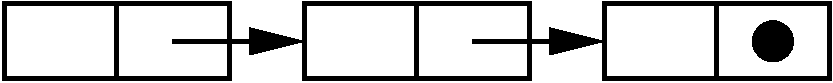
\includegraphics{../Images/llist.pdf}
%\end{center}
%\item Doubly Linked Lists:
%\begin{center}
%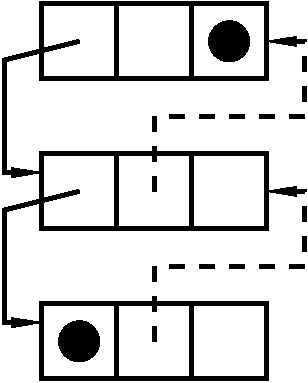
\includegraphics{../Images/dlist.pdf}
%\end{center}
%\end{itemize}
%}

\newpage
{\samepage
\begin{center}
{\Large{\bf Dynamic Trees \& Graphs}}
\end{center}
Binary Trees:
\begin{center}
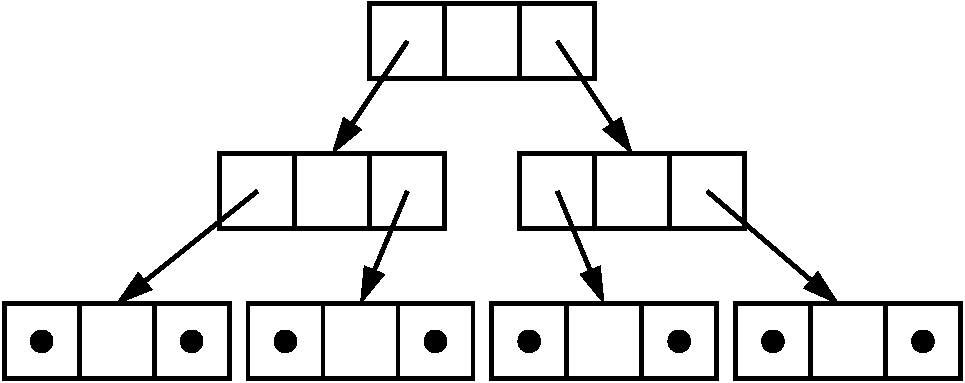
\includegraphics{../Images/tree.pdf}
\end{center}
Unidirectional Graph:
\begin{center}
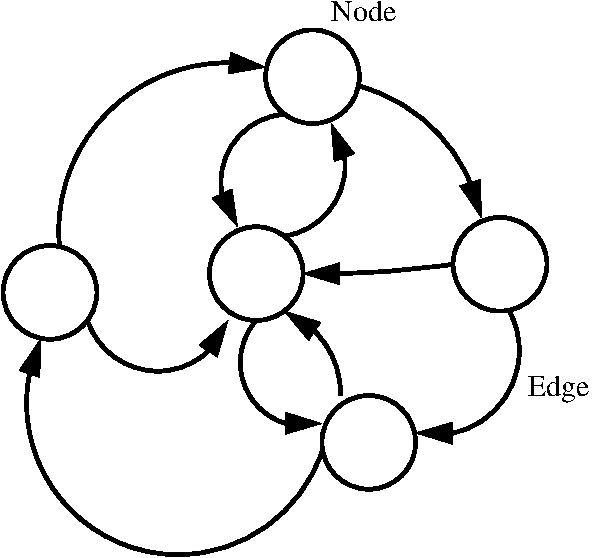
\includegraphics{../Images/graph.pdf}
\end{center}
}

\newpage
{\samepage
\begin{center}
{\Large{\bf Stacks}}
\end{center}
Push-Down Stack:
\begin{center}
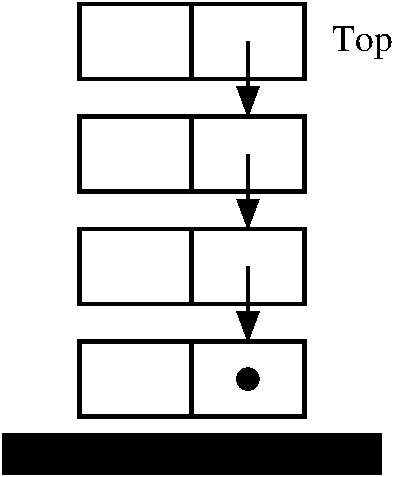
\includegraphics[scale=1.00]{../Images/stack.pdf}
\end{center}
}

\newpage
{\samepage
\begin{center}
{\Large{\bf Stacks}}
\end{center}
LIFO (Last in, First out):
\begin{center}
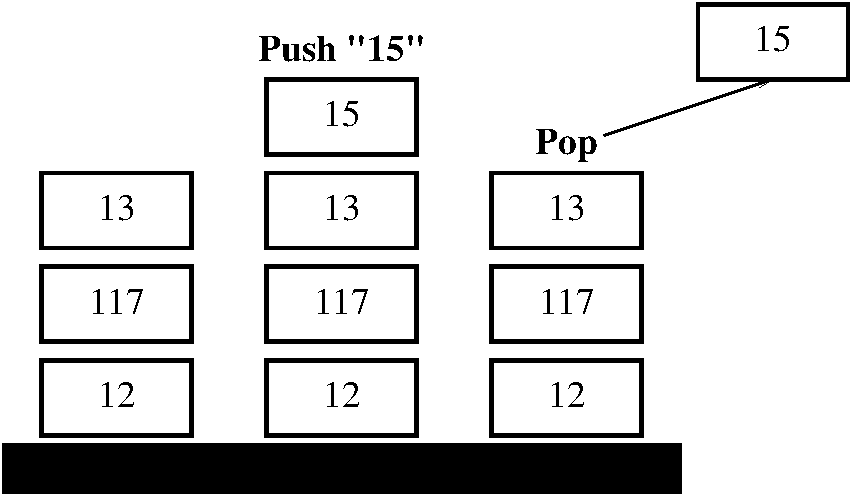
\includegraphics{../Images/pdstack.pdf}
\end{center}
\begin{itemize}
\item Operations include \verb^push^ and \verb^pop^.
\item In the C run-time system, function calls are implemented using stacks.
\item Most recursive algorithms can be re-written using stacks instead.
\item But, once again, we are faced with the question~: How best to implement such a data type~?
\end{itemize}
}

\newpage
{\samepage
\begin{center}
{\Large{\bf ADT:Stack}}
\end{center}
{\small
\begin{verbatim}
#include "../General/general.h"
typedef struct stack stack;

#include <stdio.h>
#include <stdlib.h>
#include <assert.h>
#include <string.h>

typedef enum bool {false, true} bool;

/* Create an empty stack */
stack* stack_init(void);
/* Add element to top */
void stack_push(stack* s, datatype i);
/* Take element from top */
bool stack_pop(stack* s, datatype* d);
/* Clears all space used */
bool stack_free(stack* s);

/* Optional? */

/* Copy top element into d (but don't pop it) */
bool stack_peek(stack*s,  datatype* d);
/* Make a string version for testing etc. */
void stack_tostring(stack*, char* str);
\end{verbatim}
}}

\newpage
{\samepage
\begin{center}
{\Large{\bf ADT:Stack (Realloc) I}}
\end{center}
\begin{verbatim}
typedef int datatype;
#define FORMATSTR "%d"
#define ELEMSIZE 20

#define STACKTYPE "Realloc"

#define FIXEDSIZE 16
#define SCALEFACTOR 2

struct stack {
   /* Underlying array */
   datatype* a;
   int size;
   int capacity;
};
\end{verbatim}
}

\newpage
{\samepage
\begin{center}
{\Large{\bf ADT:Stack (Realloc) II}}
\end{center}
{\small
\begin{verbatim}
#include "specific.h"
#include "../stack.h"

#define DOTFILE 5000

/* Some implementations would allow you to pass
   a hint about the initial size of the stack */
stack* stack_init(void)
{
   stack *s = (stack*) ncalloc(sizeof(stack), 1);
   s->a = (datatype*) ncalloc(sizeof(datatype),
                              FIXEDSIZE);
   s->size = 0;
   s->capacity= FIXEDSIZE;
   return s;
}

void stack_push(stack* s, datatype d)
{
   if(s==NULL){
       return;
   }
   s->a[s->size] = d;
   s->size = s->size + 1;
   if(s->size >= s->capacity){
      s->a = (datatype*) realloc(s->a,
        sizeof(datatype)*s->capacity*SCALEFACTOR);
      s->capacity = s->capacity*SCALEFACTOR;
      if(s->a == NULL){
         on_error("Stack overflow");
      }
   }
}
\end{verbatim}
}}

\newpage
{\samepage
\begin{center}
{\Large{\bf ADT:Stack (Realloc) III}}
\end{center}
\begin{verbatim}
bool stack_pop(stack* s, datatype* d)
{
   if((s == NULL) || (s->size < 1)){
      return false;
   }
   s->size = s->size - 1;
   *d = s->a[s->size];
   return true;
}

bool stack_peek(stack* s, datatype* d)
{
   if((s==NULL) || (s->size <= 0)){
      /* Stack is Empty */
      return false;
   }
   *d = s->a[s->size-1];
   return true;
}
\end{verbatim}
}

\newpage
{\samepage
\begin{center}
{\Large{\bf ADT:Stack (Realloc) IV}}
\end{center}
\begin{verbatim}
void stack_tostring(stack* s, char* str)
{
   int i;
   char tmp[ELEMSIZE];
   str[0] = '\0';
   if((s==NULL) || (s->size <1)){
      return;
   }
   for(i=s->size-1; i>=0; i--){
      sprintf(tmp, FORMATSTR, s->a[i]);
      strcat(str, tmp);
      strcat(str, "|");
   }
   str[strlen(str)-1] = '\0';
}

bool stack_free(stack* s)
{
   if(s==NULL){
      return true;
   }
   free(s->a);
   free(s);
   return true;
}
\end{verbatim}
}

\newpage
{\samepage
\begin{center}
{\Large{\bf Using the Stack}}
\end{center}
{\small
\begin{itemize}
\item We need a thorough testing program
\item Here's a version of the string reverse code for which we already seen an iterative (in-place) and a recursive solution:
\end{itemize}
\begin{verbatim}
#include "specific.h"
#include "stack.h"

int main(void)
{
   char str[100];
   unsigned int i;
   stack* s;
   datatype d;

   strcpy(str, "A man, a plan, a cat, a canal – Panama!");

   s = stack_init();
   for(i=0; i< strlen(str); i++){
      stack_push(s, str[i]);
   }
   for(i=0; i< strlen(str); i++){
      assert(stack_pop(s, &d));
      str[i] = d;
   }
   printf("%s\n", str);
   stack_free(s);
   return 0;
}
\end{verbatim}
}}

\newpage
{\samepage
\begin{center}
{\Large{\bf ADT:Stack (Dynamic) I }}
\end{center}
\begin{verbatim}
typedef int datatype;
#define FORMATSTR "%d"
#define ELEMSIZE 20
#define STACKTYPE "Linked"

struct dataframe {
   datatype i;
   struct dataframe* next;
};
typedef struct dataframe dataframe;

struct stack {
   /* Underlying array */
   dataframe* start;
   int size;
};
\end{verbatim}
}

\newpage
{\samepage
\begin{center}
{\Large{\bf ADT:Stack (Dynamic) II}}
\end{center}
{\small
\begin{verbatim}
#include "specific.h"
#include "../stack.h"

#define DOTFILE 5000

stack* stack_init(void)
{
   stack* s = (stack*) ncalloc(sizeof(stack), 1);
   return s;
}

void stack_push(stack* s, datatype d)
{
   dataframe* f;
   if(s){
      f = ncalloc(sizeof(dataframe), 1);
      f->i = d;
      f->next = s->start;
      s->start = f;
      s->size = s->size + 1;
   }

}
\end{verbatim}
}}

\newpage
{\samepage
\begin{center}
{\Large{\bf ADT:Stack (Dynamic) III}}
\end{center}
\begin{verbatim}
bool stack_pop(stack* s, datatype* d)
{
   dataframe* f;
   if((s==NULL) || (s->start==NULL)){
      return false;
   }

   f = s->start->next;
   *d = s->start->i;
   free(s->start);
   s->start = f;
   s->size = s->size - 1;
   return true;
}

bool stack_peek(stack* s, datatype* d)
{
   if((s==NULL) || (s->start==NULL)){
      return false;
   }
   *d = s->start->i;
   return true;
}
\end{verbatim}
}

\newpage
{\samepage
\begin{center}
{\Large{\bf ADT:Stack (Dynamic) IV}}
\end{center}
\begin{verbatim}
void stack_tostring(stack* s, char* str)
{
   dataframe *p;
   char tmp[ELEMSIZE];
   str[0] = '\0';
   if((s==NULL) || (s->size <1)){
      return;
   }
   p = s->start;
   while(p){
      sprintf(tmp, FORMATSTR, p->i);
      strcat(str, tmp);
      strcat(str, "|");
      p = p->next;
   }
   str[strlen(str)-1] = '\0';
}
\end{verbatim}
}

\newpage
{\samepage
\begin{center}
{\Large{\bf ADT:Stack (Dynamic) V}}
\end{center}
\begin{verbatim}
bool stack_free(stack* s)
{
   if(s){
      dataframe* tmp;
      dataframe* p = s->start;
      while(p!=NULL){
         tmp = p->next;
         free(p);
         p = tmp;
      }
      free(s);
   }
   return true;
}
\end{verbatim}
}





\newpage
{\samepage
\begin{center}
{\Large{\bf Queue}}
\end{center}
FIFO (First in, First out):
\begin{center}
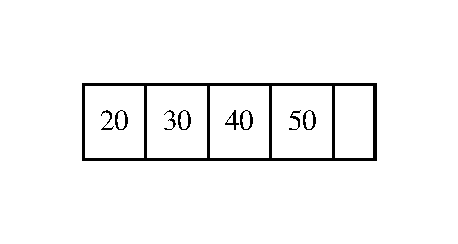
\includegraphics{../Images/Fixedq.pdf}
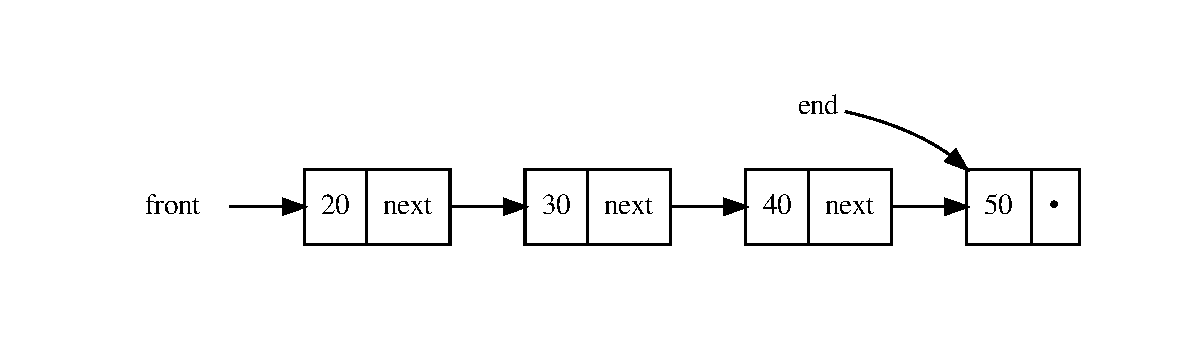
\includegraphics[width=\textwidth]{../Images/Linkedq.pdf}
\end{center}
\begin{itemize}
\item Intuitively more ``useful'' than a stack.
\item Think of implementing any kind of service (printer, web etc.)
\item Operations include \verb^enqueue^, \verb^dequeue^ and \verb^size^.
\end{itemize}
}

\newpage
{\samepage
\begin{center}
{\Large{\bf ADT:Queue}}
\end{center}
{\small
\begin{verbatim}
#include "../General/general.h"
typedef struct queue queue;

#include <stdio.h>
#include <stdlib.h>
#include <string.h>
#include <assert.h>

typedef enum bool {false, true} bool;

/* Create an empty queue */
queue* queue_init(void);
/* Add element on end */
void queue_enqueue(queue* q, datatype v);
/* Take element off front */
bool queue_dequeue(queue* q, datatype* d);
/* Return size of queue */
int queue_size(queue* q);
/* Clears all space used */
bool queue_free(queue* q);

/* Helps with visualisation & testing */
void queue_tostring(queue* q, char* str);
\end{verbatim}
} }

\newpage
{\samepage
\begin{center}
{\Large{\bf ADT:Queue (Fixed) I}}
\end{center}
{\small
\begin{verbatim}
void _inc(datatype* p);

queue* queue_init(void)
{
   queue* q = (queue*) ncalloc(sizeof(queue), 1);
   return q;
}

void queue_enqueue(queue* q, datatype d)
{
   if(q){
      q->a[q->end] = d;
      _inc(&q->end);
      if(q->end == q->front){
         on_error("Queue too large");
      }
   }
}

bool queue_dequeue(queue* q, datatype* d)
{
   if((q==NULL) || (q->front==q->end)){
      return false;
   }
   *d = q->a[q->front];
   _inc(&q->front);
   return true;
}
\end{verbatim}
} }

\newpage
{\samepage
\begin{center}
{\Large{\bf ADT:Queue (Fixed) II}}
\end{center}
{\small
\begin{verbatim}
void queue_tostring(queue* q, char* str)
{
                                                                                          int i; 
   char tmp[ELEMSIZE];

   str[0] = '\0';
   if((q==NULL) || (queue_size(q)==0)){
      return;
   }
   for(i=q->front; i != q->end;){
      sprintf(tmp, FORMATSTR, q->a[i]);
      strcat(str, tmp);
      strcat(str, "|");
      _inc(&i);
   }
   str[strlen(str)-1] = '\0';
}

int queue_size(queue* q)
{
   if(q==NULL){
      return 0;
   }
   if(q->end >= q->front){
      return q->end-q->front;
   }
   return q->end + BOUNDED - q->front;
}
\end{verbatim}
} }

\newpage
{\samepage
\begin{center}
{\Large{\bf ADT:Queue (Fixed) III}}
\end{center}
{\small
\begin{verbatim}

bool queue_free(queue* q)
{
   free(q);
   return true;
}

void _inc(datatype* p)
{
   *p = (*p + 1) % BOUNDED;
}
\end{verbatim}


\begin{center}
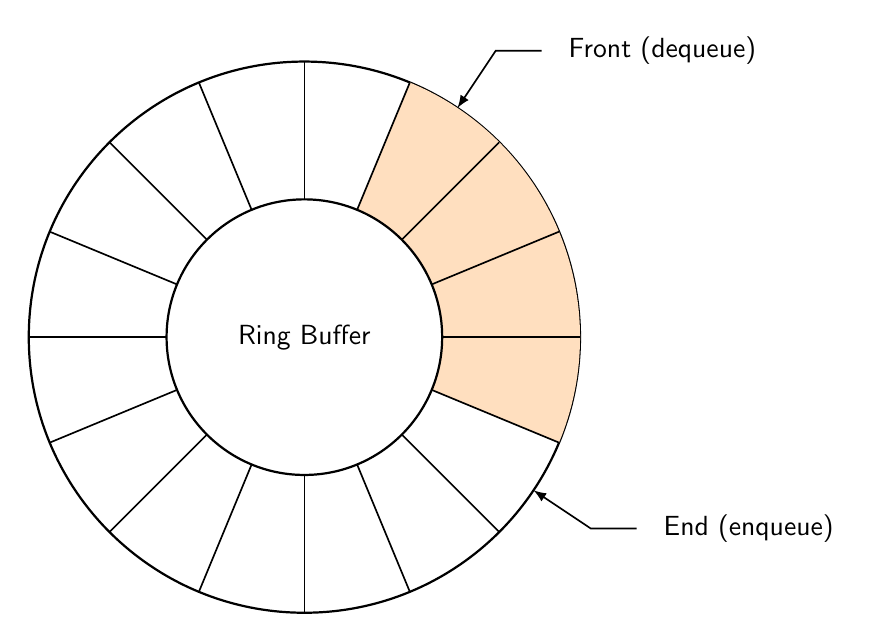
\begin{tikzpicture}[>=latex,font=\sffamily,semithick,scale=1.75]
    \draw [thick,draw=black] (0,0) circle (2);
    \fill [orange!25] (0,0) -- (67.5:2) arc [end angle=-22.5, start angle=67.5, radius=2] -- cycle;
    \foreach \angle in {90,67.5,...,-67.5}
        \draw (\angle:2) -- (\angle-180:2);
    \draw [thick,fill=white,draw=black] (0,0) circle (1);
    \node [scale=1.00] at (0,0) {Ring Buffer};
    \draw [<-] (56.25:2) -- (56.25:2.50) -- +(.333,0)
        node [right,inner xsep=.333cm] (Front) {Front (dequeue)};
    \draw [<-] (-33.75:2) -- (-33.75:2.50) -- +(.333,0)
        node [right,inner xsep=.333cm] (End) {End (enqueue)};
\end{tikzpicture}
\end{center}
} }

\newpage
{\samepage
\begin{center}
{\Large{\bf Using the Queue}}
\end{center}
{\small
\begin{itemize}
\item We need a thorough testing program
\item We'll see queues again for traversing trees
\item Simulating a (slow) printer
\end{itemize}
\begin{verbatim}
#include "specific.h"
#include "queue.h"
#include "time.h"

int main(void)
{
   queue* q;
   datatype d;
   char str[1000];

   srand(time(NULL));
   q = queue_init();
   while(queue_size(q) < 10){
      /* Slow output */
      if(rand()%10 < 1){
         queue_dequeue(q, &d);
      }
      /* Faster input */
      if(rand()%10 < 3){
         d = rand()%1000;
         queue_enqueue(q, d);
      }
      queue_tostring(q, str);
      printf("Queue : %s\n", str);
   }

   queue_free(q);
   return 0;
}
\end{verbatim}
} }

\newpage
{\samepage
\begin{center}
{\Large{\bf ADT:Queue (Dynamic) I}}
\end{center}
{\small
\begin{verbatim}
typedef int datatype;
#define FORMATSTR "%d"
#define ELEMSIZE 20

#define QUEUETYPE "Linked"

struct dataframe {
   datatype i;
   struct dataframe* next;
};
typedef struct dataframe dataframe;

struct queue {
   /* Underlying array */
   dataframe* front;
   dataframe* end;
   int size;
};
\end{verbatim}
} }

\newpage
{\samepage
\begin{center}
{\Large{\bf ADT:Queue (Dynamic) II}}
\end{center}
{\small
\begin{verbatim}
#include "specific.h"
#include "../queue.h"

queue* queue_init(void)
{
   queue* q = (queue*) ncalloc(sizeof(queue), 1);
   return q;
}

void queue_enqueue(queue* q, datatype d)
{
   dataframe* f;
   if(q==NULL){
      return;
   }

   /* Copy the data */
   f = ncalloc(sizeof(dataframe), 1);
   f->i = d;

   /* 1st one */
   if(q->front == NULL){
      q->front = f;
      q->end = f;
      q->size = q->size + 1;
      return;
   }
   /* Not 1st */
   q->end->next = f;
   q->end = f;
   q->size = q->size + 1;
}
\end{verbatim}
} }

\newpage
{\samepage
\begin{center}
{\Large{\bf ADT:Queue (Dynamic) III}}
\end{center}
{\small
\begin{verbatim}
bool queue_dequeue(queue* q, datatype* d)
{
   dataframe* f;
   if((q==NULL) ||(q->front==NULL) ||(q->end==NULL)){
      return false;
   }
   f = q->front->next;
   *d = q->front->i;
   free(q->front);
   q->front = f;
   q->size = q->size - 1;
   return true;
}

bool queue_free(queue* q)
{
   if(q){
      dataframe* tmp;
      dataframe* p = q->front;
      while(p!=NULL){
         tmp = p->next;
         free(p);
         p = tmp;
      }
      free(q);
   }
   return true;
}
\end{verbatim}
} }

\newpage
{\samepage
\begin{center}
{\Large{\bf ADT:Queue (Dynamic) IV}}
\end{center}
{\small
\begin{verbatim}
void queue_tostring(queue* q, char* str)
{
   dataframe *p;
   char tmp[ELEMSIZE];
   str[0] = '\0';
   if((q==NULL) || (q->front == NULL)){
      return;
   }
   p = q->front;
   while(p){
      sprintf(tmp, FORMATSTR, p->i);
      strcat(str, tmp);
      strcat(str, "|");
      p = p->next;
   }
   str[strlen(str)-1] = '\0';
}

int queue_size(queue* q)
{
   if((q==NULL) || (q->front==NULL)){
      return 0;
   }
   return q->size;
}
\end{verbatim}
} }

\newpage
{\samepage
\begin{center}
{\Large{\bf Detour : Graphviz}}
\end{center}
There exists a nice package, called Graphviz:
\begin{verbatim}
sudo apt install graphviz
\end{verbatim}
which allows the visualisation of graphs/dynamic structures
using the simple \verb^.dot^ language:
\begin{verbatim}
digraph {
   a -> b; b -> c; c -> a;
}
\end{verbatim}

To create a \verb^.pdf^:
\begin{verbatim}
dot -Tpdf -o graphviz.pdf examp1.dot
\end{verbatim}
\begin{center}
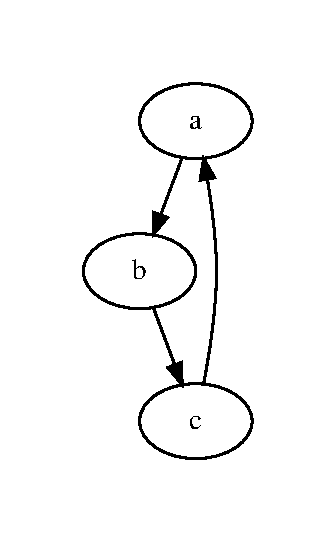
\includegraphics[scale=0.75]{../Images/graphviz.pdf}
\end{center}
}











\newpage
{\samepage
\begin{center}
{\Large{\bf Binary Trees}}
\end{center}
\begin{itemize}
\item Binary trees are used extensively in computer science
\item Game Trees
\item Searching
\item Sorting
\end{itemize}
\begin{center}
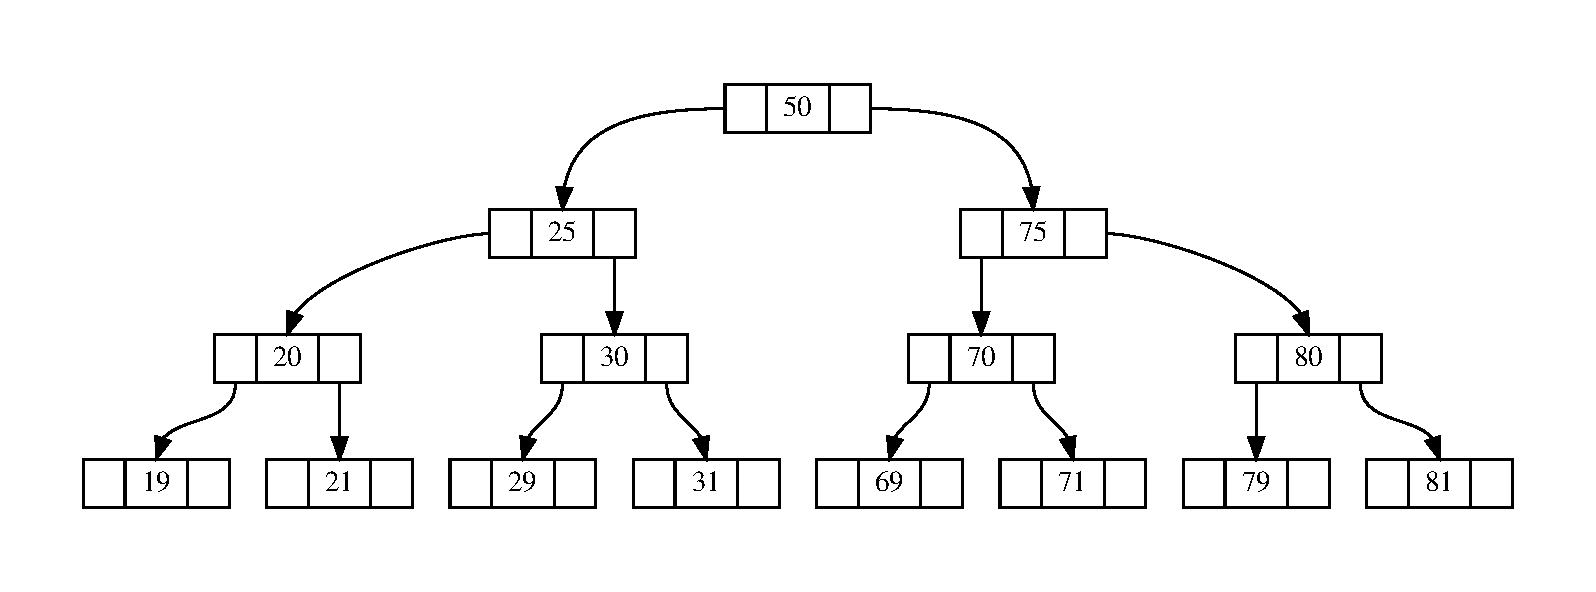
\includegraphics[width=\textwidth]{../Images/Linkedb.pdf}
\end{center}
}

\newpage
{\samepage
\begin{center}
{\Large{\bf Nomenclature}}
\end{center}
\begin{itemize}
\item Trees drawn upside-down !
\item Ancestor relationships: A is the parent of E
\item Can refer to left and right children
\item In a tree, there is only one path from the root to any child
\item A node with no children is a leaf
\item Most trees need to be created dynamically
\item Empty subtrees are set to NULL
\end{itemize}
\begin{verbatim}
typedef struct Node {
   char letter;
   struct Node *left;
   struct Node *right;
}
\end{verbatim}
}

\newpage
{\samepage
\begin{center}
{\Large{\bf Searching a Tree}}
\end{center}
This is a pre-order tree traversal:
\begin{verbatim}
Node *InTree(char l, Node *t)
{

   Node *p;

   if(t == NULL) return NULL;

   if(t->letter == l) return t;

   if((p = InTree(l, t->left)) != NULL)
      return p;

   if((p = InTree(l, t->right)) != NULL)
      return p;

   return NULL;

}
\end{verbatim}
}

\newpage
{\samepage
\begin{center}
{\Large{\bf Level Order Traversal}}
\end{center}
\begin{center}
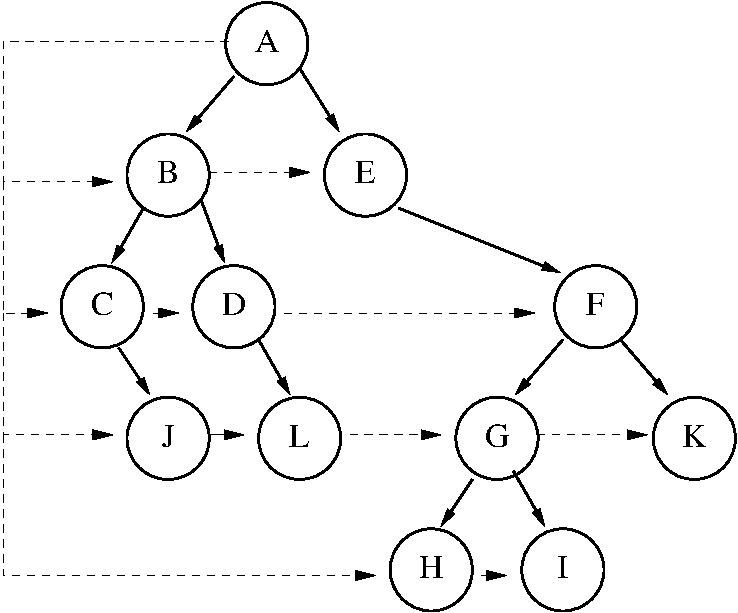
\includegraphics{../Images/treelvl.pdf}
\end{center}
To achieve this we need to use a Queue.
}

\newpage
{\samepage
\begin{center}
{\Large{\bf Queues}}
\end{center}
{\small
\begin{verbatim}
#define MAX_QUEUE 100
struct queue{
   Node *n[MAX_QUEUE];
   int front;
   int back;
};
typedef struct queue Queue;

void InitialiseQueue(Queue *q)
{
   q->front = 0;
   q->back = 0;
}

Node *Remove(Queue *q)
{
   Node *n;
   n = q->n[q->front];
   q->front = (q->front + 1)%MAX_QUEUE;
   return n;
}

void Insert(Node *t, Queue *q)
{
   q->n[q->back] = t;
   q->back = (q->back + 1)%MAX_QUEUE;
}

int Empty(Queue q)
{
   if(q.front == q.back) return 1;
   return 0;
}
\end{verbatim}
}}

\newpage
{\samepage
\begin{center}
{\Large{\bf Level Order Traversal}}
\end{center}
\begin{verbatim}
void PrintLevelOrder(Node *t)
{
   Queue q;
   Node *n;

   InitialiseQueue(&q);
   Insert(t, &q);
   while(!Empty(q)){
      n = Remove(&q);
      if(n != NULL){
         printf("%c\n", n->letter);
         Insert(n->left,  &q);
         Insert(n->right, &q);
      }
   }
}
\end{verbatim}
}

\newpage
{\samepage
\begin{center}
{\Large{\bf Complete Binary Trees\\[1.75ex]{\small(Almost Full Trees)}}}
\end{center}
Don't rush to assume a linked data structure must be used to implement
trees. If the tree is {\bf complete} (every level, except possibly the last, is completely filled, and all nodes are as far left as possible)
then an array can be used. If you ignore the first cell A[0]:

\begin{center}
\begin{tabular}{|l|l|l|}\hline
To find & Use & Iff\\ \hline
The root & $A[1]$ & $A$ is nonempty \\
The left child of $A[i]$ & $A[2i]$ & $2i \leq n$ \\
The parent of $A[i]$ & $A[i/2]$ & $i > 1$\\
Is $A[i]$ a leaf ? & True & $2i > n$\\ \hline
\end{tabular}
\end{center}

Effectively, the array is simply an encoding of the level-order traversal.
Useful for many operations, including representing {\it Heaps} (every child has a value no bigger than its parent).
}


\newpage
{\samepage
\begin{center}
{\Large{\bf Binary Search Trees}}
\end{center}
In a binary search tree the left-hand tree of a parent contains all keys less than the parent node,
and the right-hand side all the keys greater than the parent node.
\begin{center}
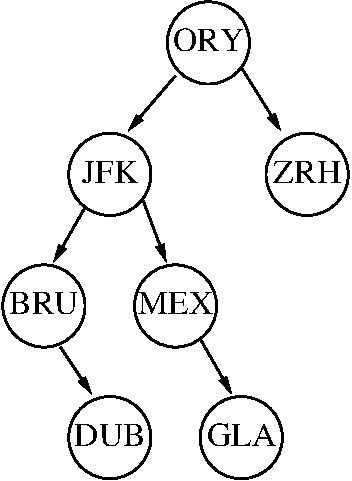
\includegraphics{../Images/treeapt.pdf}
\end{center}
}

\newpage
{\samepage
\begin{center}
{\Large{\bf Binary Search Trees}}
\end{center}
\begin{verbatim}
#include <stdio.h>
#include <stdlib.h>
#include <string.h>
#include <assert.h>
#define STRSIZE 500
struct node{
   int num;
   struct node *left;
   struct node *right;
};
typedef struct node Node;
Node *CreateNode();
char *PrintTree(Node *t);
void InsertBinTree(Node *t, int i);
int InTree(Node *t, int i);
\end{verbatim}
}

\newpage
{\samepage
\begin{center}
{\Large{\bf Binary Search Trees}}
\end{center}
\begin{verbatim}
int main(void)
{

   Node *top;
   int i;
   assert(scanf("%d", &i) == 1);
   top = CreateNode();
   top->num = i;
   while(scanf("%d", &i) == 1)
      InsertBinTree(top, i);
   printf("%s\n", PrintTree(top));
   while(scanf("%d", &i) == 1)
      printf("%d is%s in Tree\n",
         i, InTree(top, i) ? "" : " not");
   return 0;

}
\end{verbatim}
}

\newpage
{\samepage
\begin{center}
{\Large{\bf Binary Search Trees}}
\end{center}
\begin{verbatim}
void InsertBinTree(Node *t, int i)
{
   Node *p;
   if(t == NULL || i == t->num) return;
   if(i < t->num){
      if(t->left == NULL){
         p = CreateNode();
         p->num = i;
         t->left = p;
      }
      else
         InsertBinTree(t->left, i);
   }
   else{
      if(t->right == NULL){
         p = CreateNode();
         p->num = i;
         t->right = p;
      }
      else
         InsertBinTree(t->right, i);
   }
}
\end{verbatim}
}

\newpage
{\samepage
\begin{center}
{\Large{\bf Binary Search Trees}}
\end{center}
{\small
\begin{verbatim}
char *PrintTree(Node *t)
{
   char *str;

   str = calloc(STRSIZE, sizeof(char));
   assert(str != NULL);
   if(t == NULL){
      strcpy(str, "*");
      return str;
   }
   sprintf(str, "%d(%s)(%s)", t->num,
      PrintTree(t->left),
      PrintTree(t->right));
   return str;
}

int InTree(Node *t, int i)
{
   if(t == NULL) return 0;
   if(i == t->num) return 1;

   if(i < t->num)
      return InTree(t->left, i);
   else
      return InTree(t->right, i);
}
\end{verbatim}
}
}

\newpage
{\samepage
\begin{center}
{\Large{\bf Example Run}}
\end{center}
\begin{verbatim}
20
10
17
30
21
30
5
20(10(5(*)(*))(17(*)(*)))(30(21(*)(*))(*))
\end{verbatim}
}

\newpage
{\samepage
\begin{center}
{\Large{\bf Binary Search Trees}}
\end{center}
\begin{itemize}
\item  If the root of the tree is not well chosen, or the keys to be inserted are ordered, the tree can become a linked list !
\item The tree search performs best when well balanced trees are formed - large
body of literature about creating \& re-balancing trees.
\end{itemize}
}


\newpage
{\samepage
\begin{center}
{\Large{\bf Huffman Compression}}
\end{center}
\begin{itemize}
\item Often we wish to compress data, to reduce storage requirements, or to speed transmission.
\item  Text is particularly suited to compression since using one byte per character is wasteful - some letters occur much more frequently.
\item  Need to give frequently occurring letters short codes, typically a few bits. Less common letters can have long bit patterns.
\item To encode the string "BABBAGE"
\begin{center}
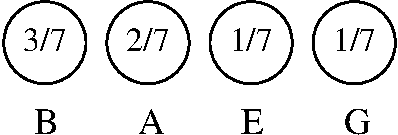
\includegraphics{../Images/huff1.pdf}
\end{center}
\end{itemize}
}

\newpage
{\samepage
\begin{center}
{\Large{\bf Huffman Compression}}
\end{center}
{\small
\begin{itemize}
\item Keep a list of characters, ordered by their frequency
\item Use the two least frequent to form a sub-tree, and re-order the nodes.
\begin{center}
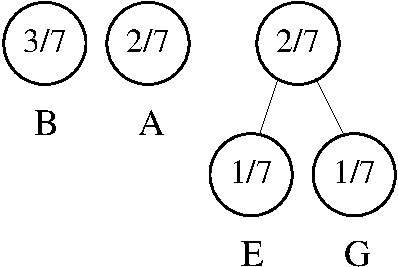
\includegraphics{../Images/huff2.pdf}
\end{center}
\begin{center}
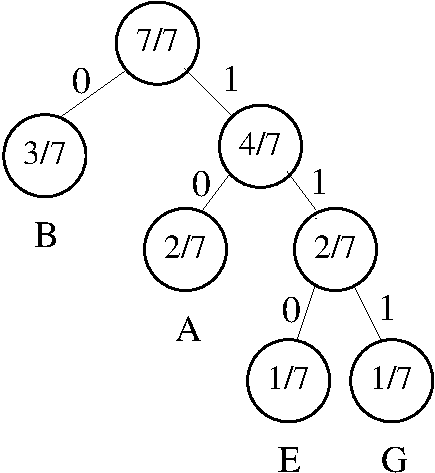
\includegraphics{../Images/huff3.pdf}
\end{center}
\item A = 10, B = 0, E = 110, G = 111
\item String stored using 13 bits.
\end{itemize}
}
}

\newpage
{\samepage
\begin{center}
{\Large{\bf Hashing}}
\end{center}
\begin{itemize}
\item To keep records of employees we might index (search) them by using
their National Insurance number: \verb^xx-##-##-##-x^
\item There are $17.6$ billion combinations (around $2^{34}$).
\item Could use an array of $17.6$ billion entries, which would make searching
for a particular entry trivial !
\item Especially wasteful since only our ($5000$) employees need to be
stored.
\item In this lecture we examine a method that, using an array of $6000$
elements, would require $2.1$ comparisons on average.
\end{itemize}
}

\newpage
{\samepage
\begin{center}
{\Large{\bf Hashing Nomenclature}}
\end{center}
{\small
\begin{itemize}
\item A hash function is a mapping, h(K), that maps from key K, onto the index of an entry.
\item A black-box into which we insert a key (e.g. NI number) and out pops an array index.
\item As an example lets use an array of size $11$ to store some airport codes, e.g.
\verb^PHL^, \verb^DCA^, \verb^FRA^.
\item In a three letter string $X_2 X_1 X_0$ the letter 'A' has the value 0, 'B' has the
value 1 etc.
\item One hash function is:
\[
h(K) = (X_2*26^2 + X_1*26 + X_0)\%11
\]
\item Applying this to "DCA":\\

$ h("DCA") = (3*26^2 + 2*26 + 0)\%11$\\

$ h("DCA") = (2080)\%11$\\

$ h("DCA") = 1 $
\end{itemize}
}}

\newpage
{\samepage
\begin{center}
{\Large{\bf Collisions}}
\end{center}
\begin{itemize}
\item Inserting "PHL", "ORY" and "GCM":
\begin{center}
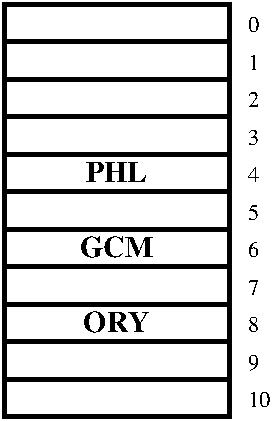
\includegraphics{../Images/hashapt.pdf}
\end{center}
\item However, inserting "HKG" causes a collision.
\begin{center}
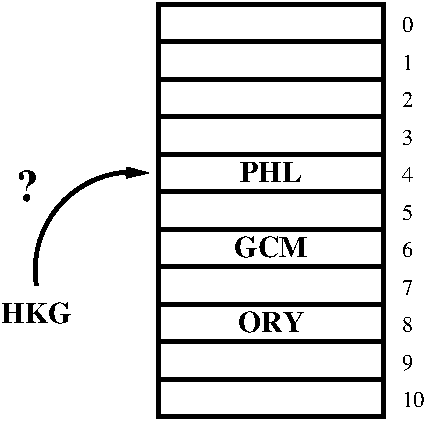
\includegraphics{../Images/hashclash.pdf}
\end{center}
\end{itemize}
}

\newpage
{\samepage
\begin{center}
{\Large{\bf Collisions}}
\end{center}
\begin{itemize}
\item An ideal hashing function maps keys into the array in a {\it uniform} and {\it random} manner.
\item Collisions occur when a hash function maps two different keys onto the same address.
\item It's very difficult to choose 'good' hashing functions.
\item Collisions are common - the {\bf von Mises} paradox. When 23 keys are randomly mapped onto 365 addresses there is a 50\% chance of a collision.
\end{itemize}
}

\newpage
{\samepage
\begin{center}
{\Large{\bf Linear Probing}}
\end{center}
{\small
\begin{center}
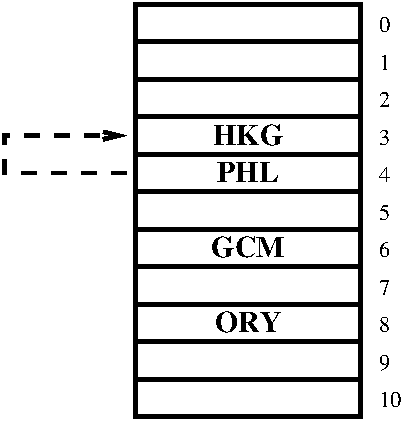
\includegraphics{../Images/hashprobe.pdf}
\begin{itemize}
\item The policy of finding another free location if a collision occurs is called open-addressing.
\item If a collision occurs then keep stepping backwards (with wrap-around) until a free location is encountered.
\item The simplest method of open-addressing is linear-probing.
\item The step taken each time (probe decrement) need not be~1.
\item Open-addressing through use of linear-probing is a very simple technique, double-hashing is generally much more successful.
\end{itemize}
\end{center}
}}

\newpage
{\samepage
\begin{center}
{\Large{\bf Double Hashing}}
\end{center}
\begin{itemize}
\item A second function p(K) decides the size of the probe decrement.
\item The function is chosen so that two keys which collide at the same address will have different probe decrements, e.g. :
{\small
\[
p(K) = MAX (1, ((X_2*26^2 + X_1*26+X_0)/11)\%11)
\]
}
\item Although "PHL" and "HKG" share the same primary hash value of $h(K)=4$, they
have different probe decrements:

$p("PHL")=4$\\

$p("HKG")=3$
\end{itemize}
}

\newpage
{\samepage
\begin{center}
{\Large{\bf Prime Array Sizes}}
\end{center}
\begin{itemize}
\item If the size of our array, $M$, was even and the probe decrement was chosen to be $2$, then only half of the locations could be probed.
\begin{center}
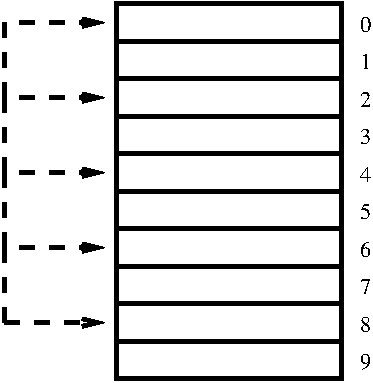
\includegraphics{../Images/hashp2.pdf}
\end{center}
\item Often we choose our table size to be a prime number and our probe decrement to be a number in the range $1 \ldots M-1$.
\item Other hashing techniques: Cuckoo Hashing
\end{itemize}
}

\newpage
{\samepage
\begin{center}
{\Large{\bf Separate Chaining}}
\end{center}
Open-addressing is not the only method of collision reduction. Another common
one is separate chaining.
\begin{center}
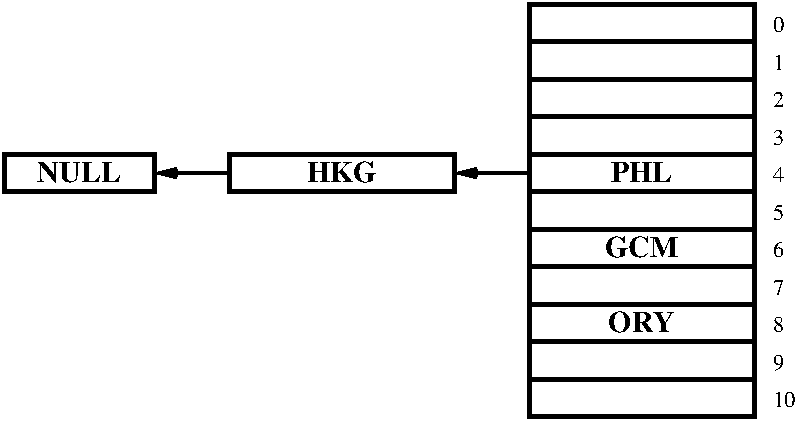
\includegraphics{../Images/hashsep.pdf}
\end{center}
}

\newpage
{\small
\begin{verbatim}
/*
Modified Bernstein hashing
5381 & 33 are magic numbers required by the algorithm
*/
int hash(unsigned int sz, char *s)
{
   unsigned long hash = 5381;
   int c;
   while((c = (*s++))){
      hash = 33 * hash ^ c;
   }
   return (int)(hash%sz);
}
\end{verbatim}

Has many similarities to the implementation of the pseudo-random number generator in C, \verb^rand()^.
{\small
\begin{verbatim}
/* This algorithm is mentioned in the ISO
   C standard, here extended for 32 bits. */
int rand_r (unsigned int *seed)
{
  unsigned int next = *seed;
  int result;

  next *= 1103515245;
  next += 12345;
  result = (unsigned int) (next / 65536) % 2048;

  ... ETC ...
\end{verbatim}
}
}

\newpage
{\samepage
\begin{center}
{\Large{\bf Sorting}}
\end{center}
\begin{itemize}
\item Bubblesort - we have seen this already, but at complexity $O(n^2)$ is
very inefficient.
\item If an algorithm uses comparison keys to decide the correct order
then the theoretical lower bound on complexity is $O(n \log n )$.
\end{itemize}
\begin{center}
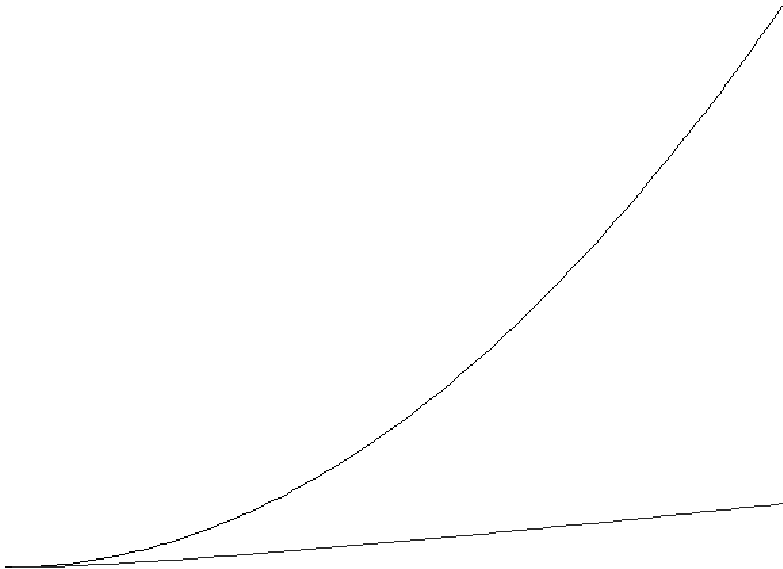
\includegraphics{../Images/nlogn.pdf}
\end{center}

}

\newpage
{\samepage
\begin{center}
{\Large{\bf Types of Sort}}
\end{center}
\begin{itemize}
\item Transposition (Bubblesort)
\item Insertion Sort (Lab Work)
\item Priority Queue (Selection sort, Heap sort)
\item Divide \& Conquer (Merge \& Quick sort)
\item Address Calculation (Proxmap)
\end{itemize}
}

\newpage
{\samepage
\begin{center}
{\Large{\bf Mergesort}}
\end{center}
The merge sort is divide-and-conquer in the sense that you
divide the array into two halves, mergesort each half and
then merge the two halves into order.
{\small
\begin{verbatim}
#include <stdio.h>
#include <stdlib.h>
#include <string.h>

void mergesort(int *src, int *spare,
               int l, int r);
void merge(int *src, int *spare, int l,
           int m, int r);

#define NUM 5000

int main(void)
{

   int i;
   int a[NUM];
   int spare[NUM];

   for(i=0; i<NUM; i++)
      a[i] = rand()%100;

   mergesort(a, spare, 0, NUM-1);

   for(i=0; i<NUM; i++)
      printf("%4d => %d\n", i, a[i]);

   return 0;

}
\end{verbatim}
}}

\newpage
{\samepage
\begin{center}
{\Large{\bf Mergesort}}
\end{center}
\begin{verbatim}
void mergesort(int *src, int *spare,
               int l, int r)
{

   int m;

   if(l != r){
      m = (l+r)/2;
      mergesort(src, spare, l, m);
      mergesort(src, spare, m+1, r);
      merge(src, spare, l, m, r);
   }

}
\end{verbatim}
}

\newpage
{\samepage
\begin{center}
{\Large{\bf Mergesort}}
\end{center}
{\small
\begin{verbatim}

void merge(int *src, int *spare,
           int l, int m, int r)
{

   int s1, s2, d;

   s1 = l;
   s2 = m+1;
   d = l;

   do{
      if(src[s1] < src[s2])
         spare[d++] = src[s1++];
      else
         spare[d++] = src[s2++];
   }while((s1 <= m) && (s2 <= r));

   if(s1 > m)
      memcpy(&spare[d], &src[s2],
             sizeof(spare[0])*(r-s2+1));
   else
      memcpy(&spare[d], &src[s1],
             sizeof(spare[0])*(m-s1+1));
   memcpy(&src[l], &spare[l],
          (r-l+1)*sizeof(spare[0]));
}
\end{verbatim}
}}

\newpage
{\samepage
\begin{center}
{\Large{\bf Quicksort}}
\end{center}
Quicksort is also divide-and-conquer. Choose some value
in the array as the {\it pivot} key. This key is used to divide
the array into two partitions. The left partition contains keys
$\leq$ pivot key, the right partition contains keys $>$ pivot.
Once again, the sort is then applied recursively.
{\small
\begin{verbatim}
#include <stdio.h>
#include <stdlib.h>
#include <math.h>

int partition(int *a, int l, int r);
void quicksort(int *a, int l, int r);

#define NUM 100000

int main(void)
{

   int i;
   int a[NUM];

   for(i=0; i<NUM; i++)
      a[i] = rand()%100;

   quicksort(a, 0, NUM-1);

   return 0;

}
\end{verbatim}
}}

\newpage
{\samepage
\begin{center}
{\Large{\bf Quicksort}}
\end{center}
\begin{verbatim}
void quicksort(int *a, int l, int r)
{

   int pivpoint;

   pivpoint = partition(a, l, r);
   if(l < pivpoint)
      quicksort(a, l, pivpoint-1);
   if(r > pivpoint)
      quicksort(a, pivpoint+1, r);

}

\end{verbatim}
}

\newpage
{\samepage
\begin{center}
{\Large{\bf Quicksort}}
\end{center}
{\small
\begin{verbatim}
int partition(int *a, int l, int r)
{

   int piv;

   piv = a[l];
   while(l<r){
      while(piv < a[r] && l<r) r--;
      if(r!=l){
         a[l] = a[r];
         l++;
      }
      /* Left -> Right Scan */
      while(piv > a[l] && l<r) l++;
      if(r!=l){
         a[r] = a[l];
         r--;
      }
   }
   a[r] = piv;
   return r;

}
\end{verbatim}
\begin{itemize}
\item Theoretically both methods have a complexity $O(n \log n)$,
although quicksort is preferred because it requires less memory and
is generally faster.
\item Quicksort can go badly wrong if the pivot key chosen is either
the maximum or minimum value in the array.
\end{itemize}
}}

\newpage
{\samepage
\begin{center}
{\Large{\bf Qsort()}}
\end{center}
Quicksort is so loved by programmers that a general version of
it exists in ANSI C. If you need an off-the-shelf sort, and speed isn't
too crucial, see \verb^man qsort^:
\begin{verbatim}
#include <stdio.h>
#include <stdlib.h>

int intcompare(const void *a, const void *b);

int main(void)
{

   int a[10];
   int i;

   for(i=0; i<10; i++){
      a[i] = 9 - i;
   }

   qsort(a, 10, sizeof(int), intcompare);

   for (i=0; i<10; i++) printf(" %d",a[i]);
   printf("\n");
   return 0;

}
\end{verbatim}
}

\newpage
{\samepage
\begin{center}
{\Large{\bf Qsort()}}
\end{center}
\begin{verbatim}
int intcompare(const void *a, const void *b)
{
    const int *ia = (const int *)a;
    const int *ib = (const int *)b;
    return *ia  - *ib;
}
\end{verbatim}
}

\newpage
{\samepage
\begin{center}
{\Large{\bf Radix Sort}}
\end{center}
\begin{itemize}
\item The radix sort is also know as the bin sort, a name
derived from its origin as a technique used on (now obsolete)
card sorters.
\item For integer data, repeated passes of radix sort focus
on the right digit (the 1's), then the second digit (the 10's)
and so on.
\item Strings can be sorted in a similar manner.
\end{itemize}
}

\newpage
{\samepage
\begin{center}
{\Large{\bf Radix Sort}}
\end{center}

459 254 472 534 649 239 432 654 477

{\bf 0}\\
{\bf 1}\\
{\bf 2} 472 432\\
{\bf 3}\\
{\bf 4} 254 534 654\\
{\bf 5}\\
{\bf 6}\\
{\bf 7} 477\\
{\bf 8}\\
{\bf 9} 459 649 239

Read out the new list:

472 432 254 534 654 477 459 649 239
}

\newpage
{\samepage
\begin{center}
{\Large{\bf Radix Sort}}
\end{center}

472 432 254 534 654 477 459 649 239

{\bf 0}\\
{\bf 1}\\
{\bf 2}\\
{\bf 3} 432 534 239\\
{\bf 4} 649\\
{\bf 5} 254 654 459\\
{\bf 6}\\
{\bf 7} 472 477\\
{\bf 8}\\
{\bf 9}
}

432 534 239 649 254 654 459 472 477

\newpage
{\samepage
\begin{center}
{\Large{\bf Radix Sort}}
\end{center}

432 534 239 649 254 654 459 472 477

{\bf 0}\\
{\bf 1}\\
{\bf 2} 239 254\\
{\bf 3}\\
{\bf 4} 432 459 472 477\\
{\bf 5} 534\\
{\bf 6} 649 654\\
{\bf 7}\\
{\bf 8}\\
{\bf 9}

239 254 432 459 472 477 534 649 654
}

\newpage
{\samepage
\begin{center}
{\Large{\bf Radix Sort}}
\end{center}
\begin{itemize}
\item This has complexity $O(n)$.
\item However this simply means that the number of operations
can be bounded by $k.n$, for some constant $k$.
\item With the radix sort, $k$
is often very large. for many lists this will be a less efficient
sort than more traditional $O(n \log n)$ algorithms.
\item It is difficult to write an all-purpose radix sort - you need
a different one for doubles, integers, strings etc.
\end{itemize}
}

\newpage
{\samepage
\begin{center}
{\Large{\bf Graphs \& Strings}}
\end{center}
\begin{itemize}
\item A graph, $G$, consists of a set of vertices (nodes), $V$, together
with a set of edges (links), $E$, each of which connects two vertices.
\begin{center}
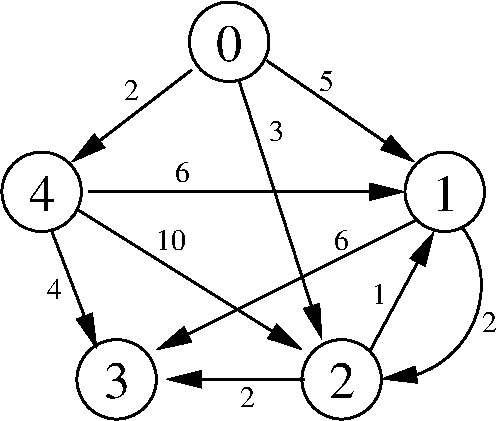
\includegraphics{../Images/grapha.pdf}
\end{center}
\item This is a directed graph (digraph).
Vertices are joined to adjacent vertices by these edges.
\item Every edge has a non-negative weight attached
which may correspond to time, distance, cost etc.
\end{itemize}
}

\newpage
{\samepage
\begin{center}
{\Large{\bf Abstract Data Types}}
\end{center}

The graph type could be implemented in a large number
of different ways.
\begin{itemize}
\item As two sets, one for vertices, one for edges.
We haven't looked at an implentation for sets, but one could use lists.
\item As an adjacency table - simply encode the weighted edges in a 2D array.
\begin{center}
\begin{tabular}{|c|ccccc|}\hline
& {\bf 0} & {\bf 1} & {\bf 2} & {\bf 3} & {\bf 4} \\ \hline
{\bf 0} & 0 & 5 & 3 & $\infty$ & 2 \\
{\bf 1} & $\infty$ & 0 & 2 & 6 & $\infty$ \\
{\bf 2} & $\infty$ & 1 & 0 & 2 & $\infty$ \\
{\bf 3} & $\infty$ &$\infty$ &$\infty$ & 0 & $\infty$ \\
{\bf 4} & $\infty$ & 6 & 10 & 4 & 0 \\ \hline
\end{tabular}
\end{center}
\end{itemize}
}

\newpage
{\samepage
\begin{center}
{\Large{\bf Abstract Data Types}}
\end{center}
\begin{itemize}
\item As a Linked list:
\begin{center}
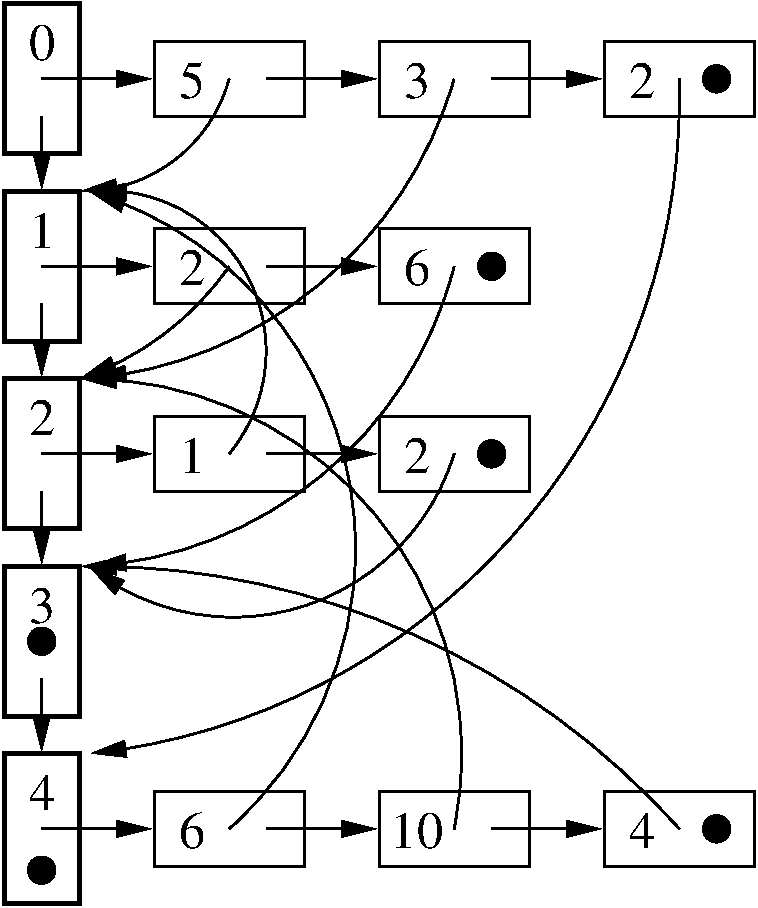
\includegraphics{../Images/graphll.pdf}
\end{center}
\end{itemize}
}

\newpage
{\samepage
\begin{center}
{\Large{\bf Shortest Path}}
\end{center}
{\small
\begin{itemize}
\item Its often important to find the shortest path through a graph
from one vertex to all others.
\item One way of doing this is the greedy algorithm.
\vspace*{-1ex}
\begin{center}
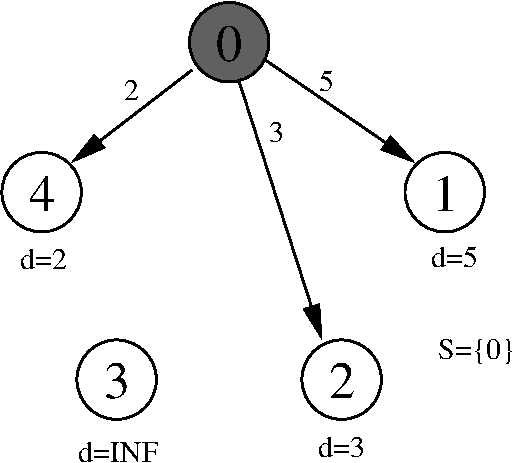
\includegraphics{../Images/graphb.pdf}
\end{center}
\vspace*{-1ex}
\begin{center}
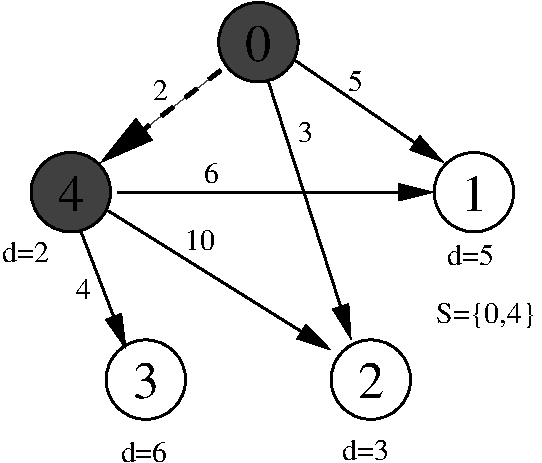
\includegraphics{../Images/graphc.pdf}
\end{center}
\end{itemize}
}}

\newpage
{\samepage
\begin{center}
{\Large{\bf Greedy Algorithm}}
\end{center}

\begin{center}
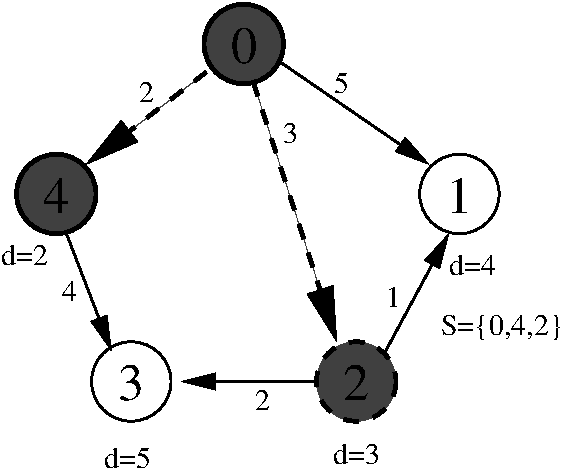
\includegraphics{../Images/graphd.pdf}
\end{center}

\begin{center}
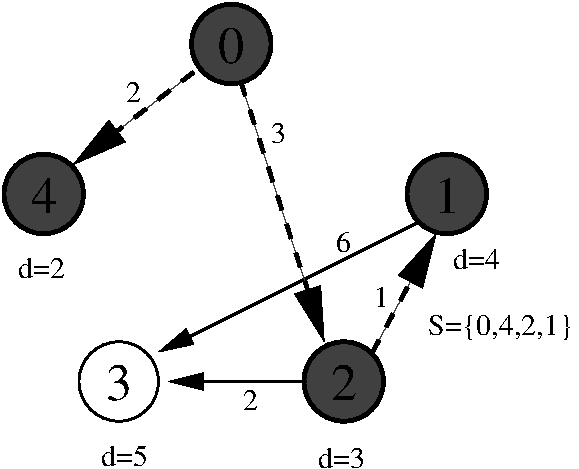
\includegraphics{../Images/graphe.pdf}
\end{center}
}

\newpage
{\samepage
\begin{center}
{\Large{\bf Greedy Algorithm}}
\end{center}

\begin{center}
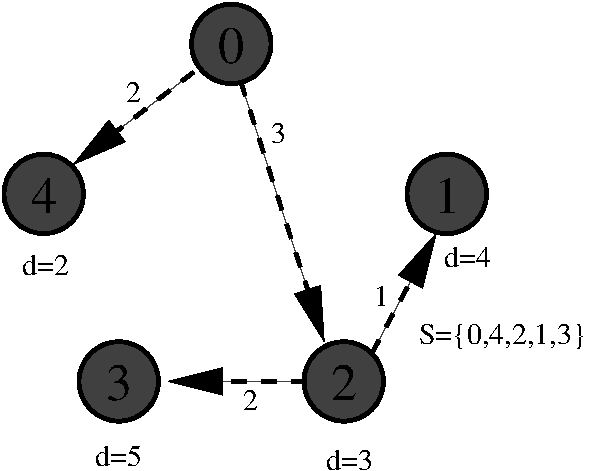
\includegraphics{../Images/graphf.pdf}
\end{center}

\begin{itemize}
\item Mark start node as distance 0.
\item Mark the closest to the start.
\item Check the closest to marked nodes.
\item Choose closest one and edges that prove it.
\end{itemize}
}

\newpage
{\samepage
\begin{center}
{\Large{\bf Greedy Algorithm}}
\end{center}
{\small
\begin{verbatim}
#include <stdio.h>
#include <limits.h>

#define INF INT_MAX
#define MAXVERTS 50

typedef enum {FALSE, TRUE} Boolean;

typedef struct graph{
        int cost[MAXVERTS][MAXVERTS];
        int n;
} Graph;

void distance(Graph g, int d[MAXVERTS]);

int main(void)
{

   int i;
   Graph g = { {{0,  5,   3,   INF, 2  },
               {INF, 0,   2,   6,   INF},
               {INF, 1,   0,   2,   INF},
               {INF, INF, INF, 0,   INF},
               {INF, 6,   10,  4,   0 }},
               5 };
   int d[MAXVERTS];

   distance(g, d);
   for(i=0; i<g.n; i++)
      printf("0=>%d dist %d\n", i, d[i]);

   return 0;

}
\end{verbatim}
}}

\newpage
{\samepage
\begin{center}
{\Large{\bf Greedy Algorithm}}
\end{center}
{\small
\begin{verbatim}
void distance(Graph g, int d[MAXVERTS])
{

   Boolean final[MAXVERTS];
   int i, w, v, min;
   final[0] = TRUE;
   d[0] = 0;
   for(v=1; v<g.n; v++){
      final[v] = FALSE;
      d[v] = g.cost[0][v];
   }
   for(i=1; i<g.n; i++){
      min = INF;
      /* Find closest v to 0 */
      for(w=1; w<g.n; w++){
         if(!final[w]){
            if(d[w] < min){
               v = w;
               min = d[w];
            }
         }
      }
      /* Add v to S */
      final[v] = TRUE;
      /* Update remaining distances in d */
      for(w=1; w<g.n; w++){
         if(!final[w]){
            if(min + g.cost[v][w] < d[w]){
               d[w] = min + g.cost[v][w];
            }
         }
      }
   }

}
\end{verbatim}
}}

%0=>0 dist 0
%0=>1 dist 4
%0=>2 dist 3
%0=>3 dist 5
%0=>4 dist 2

\newpage
{\samepage
\begin{center}
{\Large{\bf String Searching}}
\end{center}
\begin{itemize}
\item The task of searching for a string amongst a large
amount of text is commonly required in word-processors
for instance.
\item How difficult can it be ? Don't you just do a character by
character brute-force seach ?
\begin{verbatim}
Master String : AAAAAAAAAAAAH
Substring     : AAAAAAH
Substring     :  AAAAAAH
Substring     :   AAAAAAH
\end{verbatim}
\item If the master string has $m$ characters, and the search string
has $n$ characters then this search has complexity:
$O(mn)$
\end{itemize}
}

\newpage
{\samepage
\begin{center}
{\Large{\bf Rabin-Karp}}
\end{center}
{\small
Recall that to compute a hash function on a word we did something like:
\[
h("NEILL") =
\]
{\small
\[
(13\times26^4 + 4\times26^3 + 8\times26^2 + 11\times26 + 11) \% P
\]
}
where $P$ is a big prime number.
This can be expanded by Horner's method to:
{\small
\[
(((((((13\times26)+ 4)\times26) + 8)\times26) + 11)\times26 + 11) \% P
\]
}
The problem here is that for a large search string, overflow can occur.
We therefore move the {\it mod} operation inside the brackets:
{\small
\[
((((((13\times26)+ 4)\%P \times26) + 8)\%P \times26) + 11)\%P \times26 + 11) \% P
\]
}
We can compute a hash number for the search string, and for the initial
part of the master string.
When we compute the hash number for the next part of the master, most
of the computation is common, we just need to take out the effect of the first letter and add in the effect of the new one.

One small calculation each time we move one place left in the master.

Complexity $O(m+n)$ roughly, but need to check that two identical hash
numbers really has identified two identical strings.
}}

\newpage
{\samepage
\begin{center}
{\Large{\bf Rabin-Karp}}
\end{center}
{\small
\begin{verbatim}
#include <stdio.h>
#include <string.h>

#define Q 33554393
#define D 26
#define index(C) (C-'A')

int rk(char *p, char *a);

int main(void)
{
   printf("%d\n", rk("LOT", "SLOT"));
   return 0;
}
int rk(char *p, char *a)
{

   int i, dM = 1, h1=0, h2=0;
   int m = strlen(p);
   int n = strlen(a);
   for(i=1; i<m; i++) dM = (D*dM)%Q;
   for(i=0; i<m; i++){
      h1 = (h1*D+index(p[i]))%Q;
      h2 = (h2*D+index(a[i]))%Q;
   }
   /* h1 = search string hash */
   /* h2 = master hash */
   for(i=0; h1!=h2; i++){
      h2 = (h2+D*Q-index(a[i])*dM) % Q;
      h2 = (h2*D+index(a[i+m])) % Q;
      if(i>n-m) return n;
   }
   return i;
}
\end{verbatim}
}}

\newpage
{\samepage
\begin{center}
{\Large{\bf Boyer-Moore}}
\end{center}

The Boyer-Moore algorithm uses (in part) an array flagging
which characters form part of the search string and an array telling
us how far to slide right if that character appears in the master and causes
a mismatch.
{\small
\begin{verbatim}
A STRING SEARCHING EXAMPLE CONSISTING OF ...
STING    |   |    |    |    |    |
     STING   |    |    |    |    |
         STING    |    |    |    |
              STING    |    |    |
                   STING    |    |
                        STING    |
                             STING
\end{verbatim}
}
\begin{itemize}
\item With a right-to-left walk through the search string we see that
the G and the R mismatch on the first comparison. Since R doesn't appear in the
search string, we can take $5$ steps to the left.
\item The next comparison is between the G and the S. We can slide the search string right until it matches the S in the master.
\end{itemize}
}

\newpage
{\samepage
\begin{center}
{\Large{\bf Boyer-Moore}}
\end{center}
{\small
\begin{verbatim}
A STRING SEARCHING EXAMPLE CONSISTING OF ...
STING    |   |    |    |    |    |
     STING   |    |    |    |    |
         STING    |    |    |    |
              STING    |    |    |
                   STING    |    |
                        STING    |
                             STING
\end{verbatim}
}
\begin{itemize}
\item Now the C doesn't appear in the master and once again we can slide a
full $5$ places to the right.
\item After $3$ more full slides right we arrive at the T in CONSISTING.
We align the T's, and have found our match using $7$ compares (plus $5$
to verify the match).
\end{itemize}
}

\newpage
{\samepage
\begin{center}
{\Large{\bf Simple Parsing}}
\end{center}
\begin{itemize}
\item Several fundamental algorithms have been developed
to recognise legal computer programs (or expressions) and to
decompose their structure into a form more suitable for processing.
\item This operation, know as parsing, has application
beyond Computer Science, since it is directly related to the study of
the structure of languages in general.
\item In mathematics we use parentheses, brackets and
braces to indicate the boundaries of sub-expressions.
In properly formed expressions, the various types of parentheses occur in
matching pairs:
\end{itemize}
\begin{center}
{\small
\begin{verbatim}
{a*a-[(b+c)*(b+c)-(d+e)]*[sin(x-y)]}-cos(x+y)
\end{verbatim}
}
\end{center}
\begin{itemize}
\item We could use a stack to check whether or not such algebraic expressions
have properly balanced parentheses.
\end{itemize}
}

\newpage
{\samepage
\begin{center}
{\Large{\bf Simple Brackets}}
\end{center}
{\small
\begin{verbatim}
#include <stdio.h>
#include <assert.h>

/* See previous stack notes */
#include "stack.h"

#define MAXEXPR 400
void CheckBrackets(char *str);
int MatchBracket(char c, char d);

int main(void)
{

   char name[MAXEXPR];
   if(!gets(name)){
      printf("Cannot read string ?\n");
      exit(2);
   }

   CheckBrackets(name);

   return 0;

}

int MatchBracket(char c, char d)
{

   if(c == '{' && d == '}') return 1;
   if(c == '(' && d == ')') return 1;
   if(c == '[' && d == ']') return 1;

   return 0;

}
\end{verbatim}
}}

\newpage
{\samepage
\begin{center}
{\Large{\bf Simple Brackets}}
\end{center}
{\small
\begin{verbatim}
void CheckBrackets(char *str)
{

   char c;
   Stack s;
   InitialiseStack(&s);

   while(*str){

      if(*str == '{' || *str == '(' ||
         *str == '['){
         Push(&s, (int)*str);
      }
      if(*str == '}' || *str == ')' ||
         *str == ']'){
         c = Pop(&s);
         if(!MatchBracket(c, *str)){
            printf("Parse Error !\n");
            exit(2);
         }
      }
      str++;
   }

   if(!Empty(&s)){
      printf("Parse Error !\n");
      exit(2);
   }
   printf("Everything OK\n");

}
\end{verbatim}
}}

\newpage
{\samepage
\begin{center}
{\Large{\bf Reverse Polish}}
\end{center}
{\small
\begin{itemize}
\item It is a long standing tradition in mathematics to write the operator
between the operands, as in \verb^x+y^, rather than \verb^x y +^.
\item The `normal' method with the operator between the operands is
known as {\it infix} notation.
\item The alternative is called {\it Postfix} or {\it Reverse Polish}
after the Polish logician J.\ Lukasiewicz (1958) who investigated the
properties of this notation.
\item As you scan a traditional infix expression, such as:
\begin{verbatim}
A+B/C+D
\end{verbatim}
from left- to right, it is impossible to tell when you initially encounter the \verb^+^ sign whether or not you should apply the indicated operation to
A.
\item You must probe deeper into the expression to determine whether an operation with a higher priority occurs.
\item This gets very complicated.
\item Brackets make this even worse.
\end{itemize}
}}

\newpage
{\samepage
\begin{center}
{\Large{\bf Reverse Polish Notation}}
\end{center}

Infix:
\begin{verbatim}
A+B*C
A*B+C
((A+B)*C+D)/(E+F+G)
\end{verbatim}

Reverse Polish
\begin{verbatim}
ABC*+
AB*C+
AB+C*D+EF+G+/
\end{verbatim}

Notice that no brackets are required in Reverse Polish. Therefore,
for simple applications, we could require the user to enter expressions
in postfix form.
}

\newpage
{\samepage
\begin{center}
{\Large{\bf Implementing Reverse Polish}}
\end{center}
\begin{itemize}
\item Reverse Polish may be evaluated by use of a stack.
\item Examine the next character;
\item If it is a number (or variable in the general case)
push it onto the stack.
\item If it is an operator (+-/*), pop off the top two
items, perform the operation and push the result.
\item If we have reached the end the answer is the one and only
item on the stack. Else repeat.
\begin{verbatim}
8 2 5 * + 1 3 2 * + 4 - /
\end{verbatim}
\end{itemize}

\begin{center}
\begin{tabular}{|c|c|c|c|c|c|c|c|c|}\hline
   & * & + &   & * & + & - &   & $/$ \\ \hline
   &   &   & 2 &   &   &   &   &     \\
 5 &   &   & 3 & 6 &   & 4 &   &     \\
 2 & 10&   & 1 & 1 & 7 & 7 & 3 &     \\
 8 & 8 & 18& 18& 18& 18& 18& 18& 6   \\ \hline
\end{tabular}
\end{center}
}

\newpage
{\samepage
\begin{center}
{\Large{\bf Completely Parenthesised Expressions}}
\end{center}
\begin{itemize}
\item How do we convert from infix to (the more
easily handled) postfix ?
\item If your expression is comletely parenthesised:
\begin{itemize}
\item Move each operator to the space held by its
corresponding right (closing) parenthesis.
\item Remove all parentheses.
\end{itemize}
\begin{center}
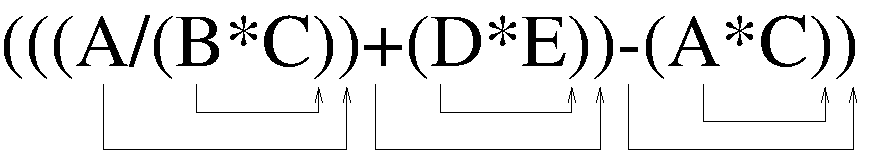
\includegraphics{../Images/cmplte.pdf}
\end{center}
\end{itemize}
}

\newpage
{\samepage
\begin{center}
{\Large{\bf Completely Parenthesised Expressions}}
\end{center}
{\small
\begin{verbatim}
#include <stdio.h>
#include <string.h>

#define MAXSTR 400

void Move(char *q, int b, char *spare);

int main(void)
{

   int brk = 0;
   char str[]="((((A+B)*C)+D)/((E+F)+G))";
   char *p = str;
   char *s;
   char *k;

   s = (char *)strdup(str);
   k = s;
\end{verbatim}
}}

\newpage
{\samepage
\begin{center}
{\Large{\bf Completely Parenthesised Expressions}}
\end{center}
{\small
\begin{verbatim}
   while(*p){
      if(*p == '(') brk++;
      if(*p == ')') brk--;
      if(*p == '*' || *p == '/' ||
         *p == '-' || *p == '+'){
         Move(p, brk, s);
         *s = ' ';
      }
      p++;
      s++;
   }
   s = k;
   while(*s){
      if(*s != '(' && *s != ' ')
         putchar(*s);
      s++;
   };
   printf("\n");

   return 0;
}
\end{verbatim}
}

\newpage
{\samepage
\begin{center}
{\Large{\bf Completely Parenthesised Expressions}}
\end{center}
\begin{verbatim}
void Move(char *q, int b, char *spare)
{

   char o;
   int brk = b-1;

   o = *q;
   do{
      q++;
      spare++;
      if(*q == '(') b++;
      if(*q == ')') b--;
   }while(*q != ')' || b != brk);
   *spare = o;

}
\end{verbatim}
}

\newpage
{\samepage
\begin{center}
{\Large{\bf General Infix to Postfix}}
\end{center}
\begin{itemize}
\item Completely parenthesised expressions are very rare, and not very general.
\item A totally general approach for translating infix to postfix relies on
a table of operator precedence:
{\large
\begin{center}
\begin{tabular}{|c|c|c|c|c|c|c|}\hline
*&$/$&+&-&(&)&\verb^'\0'^ \\ \hline
2&2&1&1&3&0&0\\\hline
\end{tabular}
\end{center}
}
\end{itemize}
}

\newpage
{\samepage
\begin{center}
{\Large{\bf General Infix to Postfix}}
\end{center}
{\small
\begin{verbatim}
#include <stdio.h>
#include <ctype.h>
#include <assert.h>
#include "stack.h"
#include "queue.h"

void PrintPostFix(char *infix);
int isoperator(char c);

int main(void)
{

   char infx[]="(((A/(B*C))+(D*E))-(A*C))";
   PrintPostFix(infx);
   return 0;

}

int isoperator(char c)
{
   if(c == '+' || c == '-' ||
      c == '*' || c == '/'){
      return 1;
   }
   else{
      return 0;
   }
}
\end{verbatim}
}}

\newpage
{\samepage
\begin{center}
{\Large{\bf General Infix to Postfix}}
\end{center}
{\small
\begin{verbatim}
void PrintPostFix(char *infix)
{

   Queue q;
   Stack s;
   int ip = 0;
   char c, d;
   int priority[256];

   InitialiseQueue(&q);
   InitialiseStack(&s);
   Push(&s, '\0');

   priority['*'] = 2; priority['/'] = 2;
   priority['+'] = 1; priority['-'] = 1;
   priority['('] = 3; priority[')'] = 0;

   do{
      c = infix[ip++];
      if(isupper(c))
         InsertQueue(c, &q);
      else if(c == ')'){
            d = Pop(&s);
            while(d != '('){
               InsertQueue(d, &q);
               d = Pop(&s);
            }
      }
      else if(c == '\0'){
               while(!EmptyStack(&s)){
                  d = Pop(&s);
                  InsertQueue(d, &q);
               }
      }
\end{verbatim}
}}

\newpage
{\samepage
\begin{center}
{\Large{\bf General Infix to Postfix}}
\end{center}
{\small
\begin{verbatim}
      else if(c == '(' || isoperator(c)){
         d = Pop(&s);
         while(priority[(int)d] >= priority[(int)c]
               && isoperator(d)){
            InsertQueue(d, &q);
            d = Pop(&s);
         }
         Push(&s, d);
         Push(&s, c);
      }
      else{
         printf("Invalid Token \"%c\"\n", c);
         exit(2);
      }
   }while(c != '\0');

   for(ip=0; !EmptyQueue(q); ip++)
      printf("%c", RemoveQueue(&q));
   printf("\n");

}
\end{verbatim}
}}

\newpage
{\samepage
\begin{center}
{\Large{\bf Formal Grammars}}
\end{center}
\begin{itemize}
\item Parsing a program is the process of grammatically analysing how it is
 composed into parts.
\item Before we can write a program to determine whether a program written in a given language is legal, we need a description of exactly what constitutes a legal program.
\item Programming languages are often described by a particular type of grammar called a {\it context free grammar}.
\item Say we wish to create a new computer language whose sole purpose is to print out noughts and ones onto the screen :
\begin{verbatim}
BEGIN
    ONE
    NOUGHT
    ONE
END
\end{verbatim}
\item We will need a formal definition of the language.
\end{itemize}
}

\newpage
{\samepage
\begin{center}
{\Large{\bf 0's \& 1's Example}}
\end{center}
{\small
\begin{verbatim}
<PROG>      ::= "BEGIN" <CODE>
<CODE>      ::= "END" | <STATEMENT> <CODE>
<STATEMENT> ::= "ONE" | "NOUGHT"
\end{verbatim}
\begin{itemize}
\item The `\verb^|^' means OR.
\item \verb^"BEGIN"^, \verb^"ONE"^ and \verb^"NOUGHT"^ are string constants.
\item \verb^<CODE>^ is described recursively.
\item You could also think of this grammar in terms of a {\it railroad diagram}:
\begin{center}
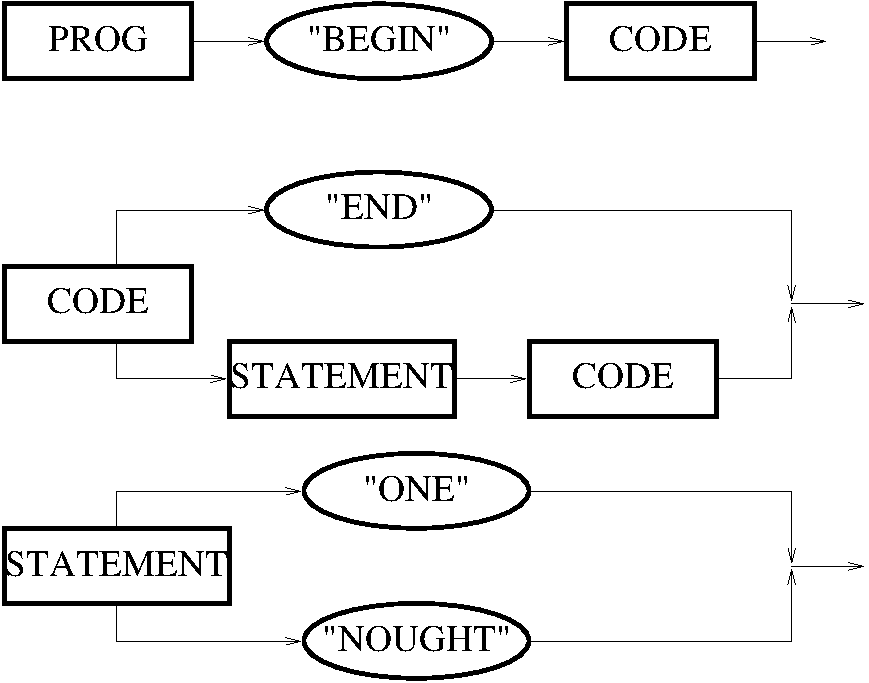
\includegraphics{../Images/railroad.pdf}
\end{center}
\end{itemize}
}}

\newpage
{\samepage
\begin{center}
{\Large{\bf 0's \& 1's Example}}
\end{center}
\begin{verbatim}
#include <stdio.h>
#include <string.h>
#include <stdlib.h>
#include <assert.h>

#define MAXNUMTOKENS 100
#define MAXTOKENSIZE 7
#define PROGNAME "01.no"
#define strsame(A,B) (strcmp(A, B)==0)
#define ERROR(PHRASE) {fprintf(stderr,
"Fatal Error %s occured in %s, line %d\n",
PHRASE, __FILE__, __LINE__); exit(2); }

struct prog{
   char wds[MAXNUMTOKENS][MAXTOKENSIZE];
   int cw; /* Current Word */
};
typedef struct prog Program;

void Prog(Program *p);
void Code(Program *p);
void Statement(Program *p);

\end{verbatim}
}

\newpage
{\samepage
\begin{center}
{\Large{\bf 0's \& 1's Example}}
\end{center}
\begin{verbatim}

int main(void)
{
   int i;
   FILE *fp;
   Program prog;

   prog.cw = 0;
   for(i=0; i<MAXNUMTOKENS; i++)
      prog.wds[i][0] = '\0';
   if(!(fp = fopen(PROGNAME, "r"))){
      fprintf(stderr, "Cannot open %s\n",
              PROGNAME);
      exit(2);
   }
   i=0;
   while(fscanf(fp, "%s", prog.wds[i++])==1
         && i<MAXNUMTOKENS);
   assert(i<MAXNUMTOKENS);
   Prog(&prog);
   printf("Parsed OK\n");
   return 0;
}
\end{verbatim}
}

\newpage
{\samepage
\begin{center}
{\Large{\bf 0's \& 1's Example}}
\end{center}
{\small
\begin{verbatim}

void Prog(Program *p)
{
   if(!strsame(p->wds[p->cw], "BEGIN"))
      ERROR("No BEGIN statement ?");
   p->cw = p->cw + 1;
   Code(p);
}

void Code(Program *p)
{
   if(strsame(p->wds[p->cw], "END"))
      return;
   Statement(p);
   p->cw = p->cw + 1;
   Code(p);
}

void Statement(Program *p)
{
   if(strsame(p->wds[p->cw], "ONE")){
      return;
   }
   if(strsame(p->wds[p->cw], "NOUGHT")){
      return;
   }
   ERROR("Expecting a ONE or NOUGHT ?");
}
\end{verbatim}
}}

\newpage
{\samepage
\begin{center}
{\Large{\bf 0's \& 1's Example}}
\end{center}
{\small
{\bf \begin{verbatim}
BEGIN
   ONE
   NOUGHT
   ONE
END
\end{verbatim}
}
\vspace*{-1.5ex}
Parsed OK

{\bf \begin{verbatim}
BEGIN ONE NOUGHT NOUGHT END
\end{verbatim} }
\vspace*{-1.5ex}
Parsed OK

{\bf \begin{verbatim}
BEGIN END
\end{verbatim} }
\vspace*{-1.5ex}
Parsed OK

{\bf \begin{verbatim}
BEGIN
  ONE
  TWO
END
\end{verbatim} }
\vspace*{-1.5ex}
Fatal Error Expecting a ONE or NOUGHT ?
occured in p01a.c, line 79

{\bf \begin{verbatim}
BEGIN
  ONE
  NOUGHT
\end{verbatim} }
\vspace*{-1.5ex}
Fatal Error Expecting a ONE or NOUGHT ?
occured in p01a.c, line 79

{\bf \begin{verbatim}
  ONE
  NOUGHT
END
\end{verbatim} }
\vspace*{-1.5ex}
Fatal Error No BEGIN statement ?
occured in p01a.c, line 55
}}

\newpage
{\samepage
\begin{center}
{\Large{\bf 0's \& 1's Example}}
\end{center}
{\small
\begin{itemize}
\item Notice that the END statement is actually used as the recursive base-case in the formal grammar in the function Code().
\item Notice that the parser doesn't actually do anything other than check that the input has the correct syntax.
\item An interpreter both checks the syntax and performs the required operations.
\item A slight modification to the code is required to produce an interpreter :
\end{itemize}
\begin{verbatim}
void Statement(Program *p)
{
   if(strsame(p->wds[p->cw], "ONE")){
      printf("1\n");
      return;
   }
   if(strsame(p->wds[p->cw], "NOUGHT")){
      printf("0\n");
      return;
   }
   ERROR("Expecting a ONE or NOUGHT ?");
}
\end{verbatim}
}}

\newpage
{\samepage
\begin{center}
{\Large{\bf Mathematical Expressions}}
\end{center}
To parse a string such as  "A+B*C", "A*(B+C)" or\\
"-(B*F)" we use :
\begin{verbatim}
<EXPR> ::= <EXPR><OP><EXPR> |
           "(" <EXPR> ")" |
           "-"<EXPR> | Letter
<OP>   ::= "+" | "-" | "*" | "/"

#include <stdio.h>
#include <ctype.h>
#include <stdlib.h>
#define MAXEXPR 400

struct prog{
        char str[MAXEXPR];
        int count;
};
typedef struct prog Prog;

void Op(Prog *p);
int isop(char c);
void Expr(Prog *p);
\end{verbatim}
}}

\newpage
{\samepage
\begin{center}
{\Large{\bf Mathematical Expressions}}
\end{center}
{\small
\begin{verbatim}
int main(void)
{

   Prog p;
   p.count = 0;

   if(scanf("%[A-Z,+,-,*,/,(,)]s", p.str) != 1){
      printf("Couldn't read your expression ?\n");
      exit(2);
   }
   Expr(&p);

   printf("Parsed OK !\n");
   return 0;

}

int isop(char c)
{

   if(c=='+' || c=='-' || c=='*' || c=='/')
      return 1;
   else
      return 0;
}

void Op(Prog *p)
{
   if(!isop(p->str[p->count])){
      printf("I was expecting a letter ?\n");
      exit(2);
   }
}
\end{verbatim}
}}

\newpage
{\samepage
{\small
\begin{verbatim}
void Expr(Prog *p)
{
   if(p->str[p->count] == '('){
      p->count = p->count + 1;
      Expr(p);
      p->count = p->count + 1;
      if(p->str[p->count] != ')'){
         printf("I was expecting a ) ?\n");
         exit(2);
      }
   }

   else if(p->str[p->count] == '-'){
      p->count = p->count + 1;
      Expr(p);
   }

   /* Note Look-Ahead */
   else if(isop(p->str[p->count+1])){
      if(isupper(p->str[p->count])){
         p->count = p->count + 1;
         Op(p);
         p->count = p->count + 1;
         Expr(p);
      }
   }
   else{
      if(!isupper(p->str[p->count]) ||
         isupper(p->str[p->count+1])){
         printf("Expected a single letter ?\n");
         exit(2);
      }
   }

}
\end{verbatim}
}
}

\newpage
{\samepage
\begin{center}
{\Large{\bf Mathematical Expressions}}
\end{center}
{\bf \begin{verbatim}
A+(B*C)
\end{verbatim}}
Parsed OK !

{\bf \begin{verbatim}
-(B*C+D)
\end{verbatim}}
Parsed OK !

{\bf \begin{verbatim}
A
\end{verbatim}}
Parsed OK !

{\bf \begin{verbatim}
A+(C*
\end{verbatim}}
I was expecting a single letter ?

{\bf \begin{verbatim}
a+c
\end{verbatim}}
Couldn't read your expression ?

{\bf \begin{verbatim}
A*B+(C*D
\end{verbatim}}
I was expecting a ) ?
}

\newpage
{\samepage
\begin{center}
{\Large{\bf Mathematical Expressions}}
\end{center}
\begin{itemize}
\item The formal grammar doesn't explain everything that the
programmer needs to know.
\item It is not clear whether the \verb^a+c^ example is
invalid or not.
\item It is not clear how spaces should be dealt with.
\end{itemize}
}

%\newpage
%{\Large
%Summary
%}
%\begin{itemize}
%\item {\it Hello World}
%\item \verb^current = current->next^
%\item The beautiful Binary Tree Search. A real
%need for recursion.
%\item von Mises paradox. The joy of hashing.
%\item Understanding why \verb^qsort()^ is $O(n\log n)$.
%\item The realisation that infix notion is evil.
%\item Anyone who wishes to
%undertake a project in Computer Vision, Image Processing, Computer
%Graphics, Robotics, or just general programming, come for a chat.
%\end{itemize}

\end{document}
